%%%%%%%%%%%%%%%%%%%%%%%%%%%%%%%%%%%%%%%%%%%%%%%%%%%%%%%%%%%%%%%%%%%%%%%%%%%%%%%%%%%%
%Do not alter this block of commands.  If you're proficient at LaTeX, you may include additional packages, create macros, etc. immediately below this block of commands, but make sure to NOT alter the header, margin, and comment settings here. 
\documentclass[12pt]{article}
 \usepackage[margin=1in, bottom=4.5cm]{geometry}
\usepackage{amsmath,amsthm,amssymb,amsfonts, enumitem, fancyhdr, color, comment, graphicx, environ, scrextend, mathtools}
\usepackage[table,dvipsnames]{xcolor}
\usepackage{tikz}  
\usepackage{tikz-3dplot} 
\usepackage{amssymb}
\usepackage{xifthen}
\pagestyle{fancy}
\setlength{\headheight}{65pt}
\newenvironment{problem}[2][Problem]{\begin{trivlist}
\item[\hskip \labelsep {\bfseries #1}\hskip \labelsep {\bfseries
#2.}]}{\end{trivlist}}
\newenvironment{lemma}[2][Lemma]{\begin{trivlist}
\item[\hskip \labelsep {\bfseries #1}\hskip \labelsep {\bfseries #2.}]}{\end{trivlist}}
\newenvironment{sol}
    {\emph{Proof.}
    }
    {
    \qed
    }
\specialcomment{com}{ \color{blue} \textbf{Comment:} }{\color{black}} %for instructor comments while grading
\NewEnviron{probscore}{\marginpar{ \color{blue} \tiny Problem Score: \BODY \color{black} }}
%%%%%%%%%%%%%%%%%%%%%%%%%%%%%%%%%%%%%%%%%%%%%%%%%%%%%%%%%%%%%%%%%%%%%%%%%%%%%%%%%

\newcommand\restr[2]{{% we make the whole thing an ordinary symbol
  \left.\kern-\nulldelimiterspace % automatically resize the bar with \right
  #1 % the function
  \vphantom{\big|} % pretend it's a little taller at normal size
  \right|_{#2} % this is the delimiter
  }}





%%%%%%%%%%%%%%%%%%%%%%%%%%%%%%%%%%%%%%%%%%%%%
%Fill in the appropriate information below
\lhead{Trey Manuszak}  %replace with your name
\rhead{MAT 473: Intermediate Real Analysis II Homework} %replace XYZ with the homework course number, semester (e.g. ``Spring 2019"), and assignment number.
%%%%%%%%%%%%%%%%%%%%%%%%%%%%%%%%%%%%%%%%%%%%%

\usepackage{blindtext}
\title{MAT 473: Intermediate Real Analysis II}
\date{Spring 2020}
\author{Trey Manuszak\\ Arizona State University}


%%%%%%%%%%%%%%%%%%%%%%%%%%%%%%%%%%%%%%
%Do not alter this block.
\begin{document}
%%%%%%%%%%%%%%%%%%%%%%%%%%%%%%%%%%%%%%


\maketitle
\newpage


%Copy the following block of text for each problem in the assignment.
\begin{problem}{1} Let $f: \mathbb{R}^2 \to \mathbb{R}$ be given by $$f(x) = \begin{cases} 
  \frac{\left|x_1\right|^a \left|x_2\right|^b}{\lVert x \rVert^c}, & \text{if } x \neq 0 \\
  0, & \text{if } x = 0, 
\end{cases}
$$ where $a,b,$ and $c$ are positive real numbers. Prove that $\lim_{x \to 0} f(x)$ exists if and only if $a + b > c$.
\end{problem}
\begin{sol}
$(\Longrightarrow):$ Suppose $a + b > c$. Then clearly $a+b-c > 0$. Then for all $x \in \mathbb{R}^2$, we have \begin{align*}
\left|\frac{\left| x_1 \right|^a\left|x_2\right|^b}{\lVert x \rVert^c} - 0\right| &= \frac{\left| x_1 \right|^a\left|x_2\right|^b}{\lVert x \rVert^c} \\ &\leq \frac{\lVert x \rVert ^a \lVert x \rVert^b}{\lVert x \rVert^c} \tag*{(By the fundamental inequalities)} \\ &= \lVert x \rVert^{a + b - c}.
\end{align*} Since $a+b-c > 0$, $\lVert x \rVert^{a+b-c}$ converges to $0$ as $x$ converges to $0$, and thus by the squeeze theorem, $\left| f(x) - 0 \right| = \left|\frac{\left| x_1 \right|^a\left|x_2\right|^b}{\lVert x \rVert^c} - 0\right|$ converges to $0$, and thus $\lim_{x \to 0} f(x) = 0$.

$(\Longleftarrow):$ Proof by contrapositive. We'll show that if $a + b \leq c$, then $\lim_{x \to 0}f(x)$ does not exist. 

\underline{Case 1}: Suppose $a + b < c$. Consider $Z = \{(t, t) : t \in \mathbb{R}^+\}$. Then, \begin{align*}
\lim_{x \to 0}\restr{f}{Z}(x) &= \lim_{t \to 0^+} \frac{\left| t \right|^a \left| t \right|^b}{\sqrt{t^2 + t^2}^c} \\ &=\lim_{t \to 0^+} \frac{t^a+b}{(\sqrt{2}t)^c} \\ &= \lim_{t \to 0^+} \frac{1}{(\sqrt{2}t)^{c-a-b}} \\ &= \infty. \tag*{(Since $c - a - b > 0$)}
\end{align*}
Thus, $\lim_{x \to 0}\restr{f}{Z}(x)$ does not exist, which implies $\lim_{x \to 0}f(x)$ does not exist.

\underline{Case 2}: Suppose $a + b = c$. Consider $Z_1 = \{(t,0) : t \in \mathbb{R}^+\}$. Then we have, \begin{align*}
\lim_{x \to 0}\restr{f}{Z_1}(x) &= \lim_{t \to 0^+}\frac{\left| t \right|^a \left| 0 \right|^b}{\sqrt{t^2 + 0}^c} \\ &= \lim_{t \to 0^+}\frac{0}{t^c} \\ &= 0.
\end{align*}
Now consider $Z_2 = \{(t,t) : t \in \mathbb{R}^+\}$. Then, \begin{align*}
\lim_{x \to 0}\restr{f}{Z_2}(x) &= \lim_{t \to 0^+}\frac{\left| t \right|^a \left| t \right|^b}{\sqrt{t^2 + 0}^c} \\ &= \lim_{t \to 0^+}\frac{t^{a+b}}{\sqrt{2}^ct^c} \\ &= \lim_{t \to 0^+} \frac{t^{a+b-c}}{\sqrt{2}^c} \\ &= \lim_{t \to 0^+} \frac{t^0}{\sqrt{2}^c} \tag*{(Since $a+b=c$)} \\ &= \frac{1}{\sqrt{2}^c}.
\end{align*}
Thus, $\lim_{x \to 0}\restr{f}{Z_1}(x) = 0 \neq \frac{1}{\sqrt{2}^c} = \lim_{x \to 0}\restr{f}{Z_2}(x)$. Thus, $\lim_{x \to 0}f(x)$ does not exist. Therefore, in all cases, $\lim_{x \to 0}f(x)$ does not exist.
\end{sol}

\begin{problem}{2}
Let $f : \mathbb{R}^2 \to \mathbb{R}$ be given by $$f(x) = \begin{cases} 
  \frac{x_1x_2^3}{x_1^2 + x_2^6}, & \text{if } x \neq 0 \\
  0, & \text{if } x = 0.
\end{cases}
$$ Prove that $\lim_{x \to 0} f(x)$ does not exist.
\end{problem}
\begin{sol}
Suppose $f : \mathbb{R}^2 \setminus \{0\} \to \mathbb{R}$. Let $Z_1 = \{(u,0)^t : u \in \mathbb{R} \setminus \{0\}\}$ and $Z_2 = \{(u^3, u)^T : u \in \mathbb{R} \setminus \{0\}\}$. We have 
\begin{align*} f(u,0) &= \frac{u \cdot 0^3}{u^2 + 0^6} = \frac{0}{u^2} = 0 \\ f(u^3,u) &= \frac{u^3 \cdot u^3}{u^6 + u^6} = \frac{u^6}{2u^6} = \frac{1}{2}.
\end{align*} Thus, $\lim_{x \to 0} \restr{f}{Z_1}(x) = 0 \neq \frac{1}{2} = \lim_{x \to 0} \restr{f}{Z_2}(x)$. Therefore, $\lim_{x \to 0} f(x)$ does not exist.
\end{sol}

\begin{problem}{3}
Let $f : \mathbb{R}^n \to \mathbb{R}^m$ be a linear function.
\begin{itemize}
\item[(a)]

Prove that $\frac{f(x)}{\lVert x \rVert}$ is a bounded function of $x$ on $\mathbb{R}^n \setminus \{0\}$. (Hint: if $f$ is represented by a matrix, then $f(x)$ equals a linear combination of the columns of that matrix.)

\vspace{1em}

\begin{sol}
Define $g:\mathbb{R}^n \setminus \{0\} \to \mathbb{R}^m$ by $g(x) = \frac{f(x)}{\lVert x \rVert}$ for all $x \in \mathbb{R}^n \setminus \{0\}$. Let $x \in \mathbb{R}^n \setminus \{0\}$. Then, \begin{align*}
\Bigg\lVert \frac{\sum_{i = 1}^m \left( \sum_{j = 1}^n f_i (e_j^{(n)})x_j\right)e_i^{(m)}}{\lVert x \rVert} \Bigg\rVert &\leq \sum_{i = 1}^m \left| \frac{\left( \sum_{j = 1}^n f_i(e_j^{(n)})x_j \right)}{\lVert x \rVert} \right| \\ &\leq \frac{\sum_{i = 1}^m \sum_{j = 1}^n \left| f_i(e_j^{(n)}) \right| \left| x_j \right|}{\lVert x \rVert} \\ &\leq \frac{\sum_{i = 1}^m \sum_{j = 1}^n \left| f_i(e_j^{(n)}) \right| \lVert x \rVert}{\lVert x \rVert} \\ &= \sum_{i = 1}^m \sum_{j = 1}^n \left| f_i(e_j^{(n)}) \right| < \infty.
\end{align*}
Thus, $\frac{f(x)}{\lVert x \rVert}$ is bounded.
\end{sol}

\item[(b)] Suppose that $f$ is not the zero map. Prove that $\lim_{x \to 0} \frac{f(x)}{\lVert x \rVert}$ does not exist. (Hint: if $f(v) \neq 0$ consider $x = tv$ for $t \in \mathbb{R} \setminus \{0\}.)$

\begin{sol}
Let $f : \mathbb{R}^n \to \mathbb{R}^m$ be a linear function that is not the zero map. Fix $v \in \mathbb{R}^n$ such that $f(v) \neq 0$. Let $Z_1 = \{kv : k \in \mathbb{R}^+\}$ and $Z_2 = \{kv : k \in \mathbb{R}^-\}$. Then, \begin{align*}
    \lim_{x \to 0} \frac{\restr{f}{Z_1}(x)}{\lVert x \rVert} &= \lim_{t \to 0^+} \frac{\restr{f}{Z_1}(tv)}{\lVert t v \rVert} \\
    &= \lim_{t \to 0^+} \frac{t\restr{f}{Z_1}(v)}{\left| t \right| \lVert v \rVert} \\
    &= \frac{\restr{f}{Z_1}(v)}{\lVert v \rVert} \cdot \lim_{t \to 0^+} \frac{t}{\left| t \right|} \\ &=  \frac{\restr{f}{Z_1}(v)}{\lVert v \rVert} \\ &> 0
\end{align*} and \begin{align*}
    \lim_{x \to 0} \frac{\restr{f}{Z_2}(x)}{\lVert x \rVert} &= \lim_{t \to 0^-} \frac{\restr{f}{Z_2}(tv)}{\lVert t v \rVert} \\
    &= \lim_{t \to 0^-} \frac{t\restr{f}{Z_2}(v)}{\left| t \right| \lVert v \rVert} \\
    &= \frac{\restr{f}{Z_2}(v)}{\lVert v \rVert} \cdot \lim_{t \to 0^-} \frac{t}{\left| t \right|} \\ &=  \frac{-\restr{f}{Z_2}(v)}{\lVert v \rVert} \\ &< 0.
\end{align*}
Thus, the limit does not exist.
\end{sol}
\end{itemize}

\end{problem}

\begin{problem}{4}
Let $V$ and $W$ be normed vector spaces. Recall that $B(V,W) = \{T \in L(V,W) : \text{sup}_{\lVert x \rVert \leq 1} \lVert Tx \rVert < \infty\}$. 

\begin{itemize}
\item[(a)] Prove that $B(V,W)$ is a vector space.

\begin{sol}
Let $V$ and $W$ be normed vector spaces. First, we'll show that $L(V,W)$ is a vector space. Suppose $T_1,T_2,T_3 \in L(V,W)$ and $\alpha, \beta \in \mathbb{K}$ and $x \in V$. Note, $L(V,W)$ is clearly closed from Definition 2.1. This leaves the following properties. \begin{itemize}
    \item[(1)] Commutativity: \begin{align*}
        (T_1 +_L T_2)(x) &= T_1x +_W T_2x \tag*{(Addition on $L(V,W)$)} \\ &= T_2x +_W T_1x \tag*{(Commutativity of addition in $W$)} \\ &= (T_2 +_L T_1)(x). \tag*{(Addition on $L(V,W)$)}
    \end{align*}
    \item[(2)] Associativity: \begin{align*}
        (T_1 +_L (T_2 +_L T_3))(x) &= T_1x +_W (T_2 +_L T_3)(x) \tag*{(Addition on $L(V,W)$)} \\ &= T_1x +_W (T_2x +_W T_3x) \tag*{(Addition on $L(V,W)$)} \\ &= (T_1x +_W T_2x) +_W T_3x \tag*{(Associativity in $W$)} \\ &= (T_1 +_L T_2)(x) +_W T_3x \tag*{(Addition on $L(V,W)$)} \\ &= ((T_1 +_L T_2) +_L T_3)(x). \tag*{(Addition on $L(V,W)$)}
    \end{align*}
    \item[(3)] Zero:  Let $0_L \in L(V,W)$ be the zero map. \begin{align*}
        (T_1 +_L 0_L)(x) &= T_1x +_W 0_Lx  \tag*{(Addition on $L(V,W)$)} \\ &= T_1x +_W 0_W \tag*{(Definition of zero map)} \\ &= T_1x. \tag*{(Addition of $0_W$)}
    \end{align*}
    \item[(4)] Additive inverse: Define $-T_1:V \to W$ by $-T_1(v) = T_1(-v)$ for all $v \in V$. Then, \begin{align*}
        (T_1 +_L -T_1)(x) &= T_1x +_W -T_1x \\ &= -T_1x +_W T_1-x \\ &= T_1(x +_V(-x))  \tag*{(Linearity of $T_1$)} \\ &= T_1 \cdot 0_V \tag*{(Addititive inverse in $V$)} \\ &= 0_W. \tag*{(Linearity of $T_1$)}
    \end{align*}
    Since $x \in V$ was arbitrary, this is true for all $x \in V$. Thus, $T_1 +_L -T_1 = 0_L$.
    \item[(5)] Multiplication over $\mathbb{K}$: \begin{align*}
        \alpha \cdot (\beta \cdot T_1 (x)) &= \alpha \cdot (\beta T_1x) \tag*{(Definition of $T_1$)} \\ &= \alpha \beta (T_1x) \tag*{(Multiplication over $\mathbb{K}$ in $W$)} \\ &= ((\alpha \beta ) \cdot T_1)(x). \tag*{(Definition of $T_1$)}
    \end{align*}
    \item[(6)] Unit of scalar multiplication: \begin{align*}
        (1 \cdot T_1)(x) &= 1 \cdot T_1(x) \tag*{(Linearity of scalar multiplication)} \\ &= T(x). \tag*{(Definition of 1)}
    \end{align*}
    \item[(7)] Distribution of scalar multiples: \begin{align*}
        (\alpha(T_1 +_L T_2))(x) &= \alpha((T_1 +_L T_2)(x)) \tag*{(Linearity of scalar multiplication)} \\ &= \alpha (T_1x +_W T_2x) \tag*{(Addition on $L(V,W)$)} \\ &= \alpha T_1x +_W \alpha T_2x \tag*{(Distribution of scalar multiples on $W$)} \\ (\alpha T_1 +_L \alpha T_2)(x) &= (\alpha T_1)x +_W (\alpha T_2)x \tag*{(Addition on $L(V,W)$)} \\ &= \alpha T_1x +_W \alpha T_2x. \tag*{(Scalar multiplication on $L(V,W)$)}
    \end{align*}
\end{itemize} 
Therefore, $L(V,W)$ is a vector space. 

\hspace{1em} Now, we'll show $B(V,W)$ is closed and thus a subspace of $L(V,W)$. Let $T_1, T_2 \in B(V,W)$ and $\alpha, \beta \in \mathbb{K}$ and $x \in V$. Then, \begin{align*}
    \sup_{\lVert x \rVert \leq 1} \lVert (\alpha T_1 +_B \beta T_2)(x) \rVert &\leq \sup_{\lVert x \rVert \leq 1} (\left| \alpha \right| \lVert T_1x \rVert + \left| \beta \right| \lVert T_2x \rVert) \tag*{(By triangle inequality)} \\ &\leq \left| \alpha \right| \sup_{\lVert x \rVert \leq 1} \lVert T_1x \rVert + \left| \beta \right| \sup_{\lVert x \rVert \leq 1} \lVert T_2x \rVert \tag*{(Definition of supremum)} \\ &= \left| \alpha \right| \lVert T_1 \rVert + \left| \beta \right| \lVert T_2 \rVert \tag*{(Definition of $\lVert T_1 \rVert$ and $\lVert T_2 \rVert$)} \\ &< \infty.
\end{align*}
Thus, $(\alpha T_1 +_B \beta T_2) \in B(V,W)$, which implies $B(V,W)$ is a subspace of $L(V,W)$. Therefore, $B(V,W)$ is a vector space.
\end{sol}

\item[(b)] For $T \in B(V,W)$, let $\lVert T \rVert = \text{sup}_{\lVert x \rVert \leq 1} \lVert Tx \rVert$. Prove that $\lVert \cdot \rVert$ is a norm on $B(V,W)$.

\begin{sol}
Since $\lVert T_1x \rVert_W \geq 0$ for all $x \in V$ by positivity of $\lVert \cdot \rVert_W$, we have $\sup_{\lVert x \rVert \leq 1} \lVert T_1x \rVert_W \geq 0$. Now suppose $\lVert T_1 \rVert = 0$. Then $\sup_{\lVert x \rVert \leq 1} \lVert T_1x \rVert = 0$. Suppose to the contrary there exists $v \in V$ such that $\lVert T_1v \rVert > 0$. Then since $\sup_{\lVert x \rVert \leq 1} \lVert T_1x \rVert = 0$, $\lVert v \rVert > 1$. But then $\lVert \frac{v}{\lVert v \rVert} \rVert = 1$, so $\lVert T_1 \frac{v}{\lVert v \rVert} \rVert = 0$. But, then $\lVert T_1 \frac{v}{\lVert v \rVert} \rVert = \left| \frac{1}{\lVert v \rVert} \right| \lVert T_1v \rVert = 0$, which implies $\lVert T_1v \rVert = 0$. This is a contradiction. Therefore, $T_1$ is the zero map and we have positivity of $\lVert \cdot \rVert$.

\hspace{1 em} Next, \begin{align*}
    \lVert \alpha T_1 \rVert &= \sup_{\lVert x \rVert \leq 1} \lVert \alpha T_1x \rVert \tag*{(Definition of $\lVert \alpha T_1 \rVert$)} \\ &= \left| \alpha \right| \sup_{\lVert x \rVert \leq 1} \lVert T_1x \rVert \tag*{(Homogeneity of supremum norm)} \\ &= \left| \alpha \right| \lVert T_1 \rVert. \tag*{(Definition of $\lVert T_1 \rVert$)}
\end{align*} 
Thus, we have homogeneity of $\lVert \cdot \rVert$. 

\hspace{1 em} Lastly, \begin{align*}
    \lVert T_1 +_B T_2 \rVert &= \sup_{\lVert x \rVert \leq 1} \lVert (T_1 +_B T_2)(x) \rVert \tag*{(Definition of $\lVert T_1 +_B T_2 \rVert$)} \\ &\leq \sup_{\lVert x \rVert \leq 1} (\lVert T_1x \rVert + \lVert T_2x \rVert ) \tag*{(Triangle inequality of the norm on $W$)} \\ &\leq \sup_{\lVert x \rVert \leq 1} \lVert T_1x \rVert + \sup_{\lVert x \rVert \leq 1} \lVert T_2x \rVert \tag*{(Property of supremum norm)} \\ &= \lVert T_1 \rVert + \lVert T_2 \rVert. \tag*{(Definition of $\lVert T_1 \rVert$ and $\lVert T_2 \rVert$)}
\end{align*}
Thus, we have the triangle inequality of $\lVert \cdot \rVert$. Therefore, $\lVert \cdot \rVert$ is a norm on $B(V,W)$.
\end{sol}
\end{itemize}
\end{problem}

\begin{problem}{5} 
  Let $f : M_{m \times n} \to M_n$ be given by $f(A) = A^tA$. Prove that $f$ is differentiable, and find a formula for $f'(A)$. (Hint: use facts about the operator norm and the transpose of a matrix.)
  \end{problem}
  \begin{sol}
  Let $f : M_{m \times n} \to M_n$ be given by $f(A) = A^tA$. Let $A \in M_{m \times n}$. Define $T \in B(M_{m \times n}, M_n)$ by $T(h) = A^th + h^tA$. Also, define $\lVert \cdot \rVert_E$ as the Euclidean norm and $\lVert \cdot \rVert_O$ as the operator norm.  Then \begin{align*}
      \lim_{h \to 0} \frac{\lVert f(A + h) - f(A) - T(h)\rVert_O}{\lVert h \rVert_O} &= \lim_{h \to 0} \frac{\lVert (A+h)^t(A+h) - A^tA - A^th - h^tA \rVert_O}{\lVert h \rVert_O} \tag*{(Definition of $f$ and $T$)} \\ &= \lim_{h \to 0} \frac{\lVert (A+h)^tA + (A+h)^th - A^tA - A^th - h^tA \rVert_O}{\lVert h \rVert_O} \tag*{(By distribution)} \\ &= \lim_{h \to 0} \frac{\lVert (A^t+h^t)A + (A^t+h^t)h - A^tA - A^th - h^tA \rVert_O}{\lVert h \rVert_O} \tag*{(Property of transpose)} \\ &= \lim_{h \to 0} \frac{\lVert A^tA+h^tA + A^th+h^th - A^tA - A^th - h^tA \rVert_O}{\lVert h \rVert_O} \tag*{(By distribution)} \\ &= \lim_{h \to 0} \frac{\lVert h^th \rVert_O}{\lVert h \rVert_O} \tag*{(By subtraction)} \\ &\leq \frac{\lVert h^t \rVert_O \cdot \lVert h \rVert_O}{\lVert h \rVert_O} \tag*{(Property of operator norm)} \\ &= \lim_{h \to 0} \frac{\lVert h \rVert_O^2}{\lVert h \rVert_O} \tag*{(Property of operator norm)} \\ &= \lim_{h \to 0} \lVert h \rVert_O \\ &= 0.
  \end{align*}
  Since $0 \leq \lim_{h \to 0} \frac{\lVert f(A + h) - f(A) - T(h)\rVert_O}{\lVert h \rVert_O}$, then by squeeze theorem, $\lim_{h \to 0} \frac{\lVert f(A + h) - f(A) - T(h)\rVert_O}{\lVert h \rVert_O} = 0$. Also, we know that, $\lim_{h \to 0} \frac{f(A+h) - f(A) - T(h)}{\lVert h \rVert_E} = 0 \Longleftrightarrow\lim_{h \to 0} \frac{\lVert f(A + h) - f(A) - T(h)\rVert_E}{\lVert h \rVert_E} = 0$. Thus, since $A \in M_{m \times n} = \mathbb{R}^{mn}$, then any two norms are comparable by Corollary 2.11, which implies there exists $k_1,k_2 \in \mathbb{R}$ such that for all $x \in \mathbb{R}$, $\lVert x \rVert_0 \leq k_1 \cdot \lVert x \rVert_E$ and $\lVert x \rVert_E \leq k_2 \cdot \lVert x \rVert_O$. Then, we get \begin{align*}
      \lim_{h \to 0} \frac{\lVert f(A+h) - f(A) - T(h) \rVert_E}{\lVert h \rVert_E} &\leq \lim_{h \to 0} \frac{k_2 \lVert f(A+h) - f(A) - T(h) \rVert_O}{\frac{1}{k_1}\lVert h \rVert_O} \tag*{(By comparability of $\lVert \cdot \rVert_E$ and $\lVert \cdot \rVert_O$)} \\ &= k_1k_2 \lim_{h \to 0} \frac{\lVert f(A+h) - f(A) - T(h) \rVert_O}{\lVert h \rVert_O} \tag*{(Property of limits)} \\ &= k_1k_2 \cdot 0 \\ &= 0.
  \end{align*}
  Since, $0 \leq \lim_{h \to 0} \frac{\lVert f(A+h) - f(A) - T(h) \rVert_E}{\lVert h \rVert_E}$, then by squeeze theorem, $\lim_{h \to 0} \frac{\lVert f(A+h) - f(A) - T(h) \rVert_E}{\lVert h \rVert_E} = 0$. This implies, $\lim_{h \to 0} \frac{f(A+h) - f(A) - T(h)}{\lVert h \rVert_E} = 0$. Thus, $f$ is differentiable at $A$. However, since $A$ was arbitrary, then $f$ is differentiable for all $A \in M_{m \times n}$. Therefore, $f'(A)(h) = A^th + h^tA$.
  \end{sol}
  
  \begin{problem}{6} 
  Let $f: \mathbb{R}^2 \to \mathbb{R}$ be given by $$f(x) = \begin{cases} 
       \frac{x_1^2 x_2}{\lVert x \rVert^2}, & \text{if } x \neq 0 \\
        0, & \text{if } x = 0. 
     \end{cases}
  $$ Prove that all directional derivatives of $f$ exist at 0, and that $D_vf(0)$ is not a linear function of $v$.
  \end{problem}
  \begin{sol}
  Let $f: \mathbb{R}^2 \to \mathbb{R}$ be given by $$f(x) = \begin{cases} 
       \frac{x_1^2 x_2}{\lVert x \rVert^2}, & \text{if } x \neq 0 \\
        0, & \text{if } x = 0. 
     \end{cases}
  $$ Let $v \in \mathbb{R}^2 \setminus (0, 0)$. Then, \begin{align*}
      D_vf(0) &= \lim_{t \to 0} \frac{f(0 + tv) - f(0)}{t} \tag*{(Definition of $D_vf(x)$ in $\mathbb{R}^2$)} \\ &= \lim_{t \to 0} \frac{\frac{(tv_1)^2(tv_2)}{\lVert tv \rVert^2} - 0}{t} \tag*{(Definition of $f$} \\ &= \lim_{t \to 0} \frac{t^2v_1^2tv_2}{t\sqrt{(tv_1)^2+(tv_2)^2}^2} \tag*{(Definition of Euclidean norm)} \\ &= \lim_{t \to 0} \frac{t^2v_1^2v_2}{t^2v_1^2 + t^2v_2^2} \\ &= \lim_{t \to 0} \frac{t^2v_1^2v_2}{t^2(v_1^2 + v_2^2)} \tag*{(by factoring $t^2$)} \\ &= \lim_{t \to 0} \frac{v_1^2v_2}{v_1^2 + v_2^2}.
  \end{align*}
  Also, we have \begin{align*}
      D_{(0, 0)}f(0) &= \lim_{t \to 0} \frac{f(0 + t \cdot 0) - f(0)}{t} \\ &= \lim_{t \to 0} \frac{0}{t} \\ &= 0.
  \end{align*}
  So, we have $D_vf(0):\mathbb{R}^2 \to \mathbb{R}$ defined by $$D_vf(0) = \begin{cases} 
       \frac{v_1^2 v_2}{v_1^2 + v_2^2}, & \text{if } v \neq 0 \\
        0, & \text{if } v = 0. 
     \end{cases}$$
  Consider $p = (1, 0)$ and $q = (0, 1)$. Then, $D_pf(0) = \frac{1^2 \cdot 0}{1^2 + 0^2} = 0$ and $D_qf(0) = \frac{0^2 \cdot 1}{0^2 + 1^2} = 0$, and $D_{p + q}f(0) = \frac{1^2 \cdot 1}{1^2 + 1^2} = \frac{1}{2}$. Therefore, $D_vf(0)$ is not linear since $D_{p + q}f(0) = \frac{1}{2} \neq 0 = 0 + 0 = D_pf(0) + D_qf(0)$.
  \end{sol}
  
  \begin{problem}{7}
  Let $f: \mathbb{R}^2 \to \mathbb{R}$ be given by $$f(x) = \begin{cases} 
       \frac{x_1 x_2^3}{x_1^2 + x_2^4}, & \text{if } x \neq 0 \\
        0, & \text{if } x = 0. 
     \end{cases}
  $$ Prove that all directional derivatives of $f$ exist at 0, that $D_vf(0)$ is a linear function of $v$, and that $f$ is not differentiable at 0.
  \end{problem}
  \begin{sol}
  Let $f: \mathbb{R}^2 \to \mathbb{R}$ be given by $$f(x) = \begin{cases} 
       \frac{x_1 x_2^3}{x_1^2 + x_2^4}, & \text{if } x \neq 0 \\
        0, & \text{if } x = 0. 
     \end{cases}
  $$ Let $v \in \mathbb{R}^2 \setminus (0, 0)$. Then, we have \begin{align*}
      D_vf(0) &= \lim_{t \to 0} \frac{f(0 + tv) - f(0)}{t} \\ &= \lim_{t \to 0} \frac{\frac{tv_1(tv_2)^3- 0}{(tv_1)^2 + (tv_2)^4}}{t} \tag*{(Definition of $f$)} \\ &= \lim_{t \to 0} \frac{t^3v_1v_2}{t^2v_1^2 + t^4v_2^4} \\ &= \lim_{t \to 0} \frac{tv_1v_2}{v_1^2 + t^2v_2^4} \\ &= \frac{0}{v_1^2} \\ &= 0.
  \end{align*}
  Also note that $$
      D_0f(0) = \lim_{t \to 0} \frac{f(0 + t \cdot 0) - f(0)}{t} = \lim_{t \to 0} \frac{0}{t} = 0.$$ Thus, $D_vf(0):\mathbb{R}^2 \to \mathbb{R}$ is defined by $D_vf(0) = 0$, which is linear since it is the zero map. Also, the Jacobian matrix of $f$ evaluated at $0$ is $(0, 0)$. To see if $f$ is differentiable at $0$, we have that \begin{align*}
          \lim_{h \to 0} \frac{f(0 + h) - f(0) - (0, 0)\cdot h}{\lVert h \rVert} = \lim_{h \to 0} \frac{\frac{h_1h_2^3}{h_1^2 + h_2^4}}{\sqrt{h_1^2 + h_2^2}}.
      \end{align*}
      Consider $Z_1 = \{(t^2, t) : t \in \mathbb{R}^+\}$. Then, \begin{align*}
          \lim_{h \to 0} \restr{\frac{h_1h_2^3}{(h_1^2 + h_2^4)\sqrt{h_1^2 + h_2^2}}}{Z_1} &= \lim_{t \to 0^+} \frac{t^2t^3}{(t^4 + t^4)\sqrt{t^4 + t^2}} \\ &= \lim_{t \to 0^+} \frac{t}{2\sqrt{t^4 + t^2}} \\ &= \lim_{t \to 0} \sqrt{\frac{t^2}{4t^4t^2}} \\ &= \sqrt{\frac{1}{4t^2 + 4}} \\ &= \frac{1}{2}.
      \end{align*}
      This means that the limit is $\frac{1}{2}$ or does not exist. However, since it is not equal to 0 either way, the derivative does not exist at 0.
  \end{sol}
  
  \begin{problem}{8} 
  Let $E = \{x \in \mathbb{R}^2 : x_1 > 0 \text{ and } 0 < x_2 < x_1^2\}$. Define $f : \mathbb{R}^2 \to \mathbb{R}$ by  $$f(x) = \begin{cases} 
       1, & \text{if } x \in E \\
        0, & \text{if } x \not\in E. 
     \end{cases}
  $$ ($f$ is called the \textit{characteristic function} of the set $E$.) Prove that all directional derivatives of $f$ exist at 0, and equal 0, but that $f$ is not differentiable at 0.
  \end{problem}
  \begin{sol}
  Let $E = \{x \in \mathbb{R}^2 : x_1 > 0 \text{ and } 0 < x_2 < x_1^2\}$. Define $f : \mathbb{R}^2 \to \mathbb{R}$ by  $$f(x) = \begin{cases} 
       1, & \text{if } x \in E \\
        0, & \text{if } x \not\in E. 
     \end{cases}
  $$ Define $A = \{x \in \mathbb{R}^2 : x_1 > 0 \text{ and } x_2 > 0 \text{ or } x_1 < 0 \text{ and } x_2 < 0\}$. Let $v \in A$ be arbitrary. 
  
  \vspace{1em}
  \noindent\underline{Case 1}: Suppose $v_1 > 0$ and $v_2 > 0$. 
  
  Since $(tv_1) < 0$ for all $t < 0$, which implies $tv \not\in E$, we have, $$\lim_{t \to 0^-} \frac{f(0 + tv) - f(0)}{t} = \lim_{t \to 0^-} \frac{f(tv)}{t} = \lim_{t \to 0^-} \frac{0}{t} = 0,$$ which implies $f(tv) = 0$. Let $\delta \in \mathbb{R}$ such that $0 < \delta < \frac{v_2}{v_1^2}$. By multiplication of $\delta v_1^2 > 0$, $0 < (\delta v_1)^2 < \delta v_2$. This means, $\delta v \not \in E$. Thus, for all $0 < t \leq \frac{v_2}{v_1^2}$, $$\lim_{t \to 0^+} \frac{f(0 + tv) - f(0)}{t} = \lim_{t \to 0^+} \frac{f(tv)}{t} = \lim_{t \to 0^+} \frac{0}{t} = 0,$$ which implies $f(tv) = 0$.
  
  \vspace{1em}
  \noindent\underline{Case 2}: Suppose $v_1 < 0$ and $v_2 < 0$. 
  
  Since $(tv_1) < 0$ for all $t > 0$, which implies $tv \not\in E$, we have, $$\lim_{t \to 0^+} \frac{f(0 + tv) - f(0)}{t} = \lim_{t \to 0^+} \frac{f(tv)}{t} = \lim_{t \to 0^+} \frac{0}{t} = 0,$$ which implies $f(tv) = 0$. Let $\phi \in \mathbb{R}$ such that $\frac{v_2}{v_1^2} < \phi < 0$. By multiplication of $\phi v_1^2 < 0$, $\phi v_2 > (\phi v_1)^2 > 0$, which implies $\phi v \not\in E$. Then, for all $\frac{v_2}{v_1^2} \leq t < 0$, we have $$\lim_{t \to 0^-} \frac{f(0 + tv) - f(0)}{t} = \lim_{t \to 0^-} \frac{f(tv)}{t} = \lim_{t \to 0^-} \frac{0}{t} = 0,$$ which implies $f(tv) = 0$.
  
  Therefore, since in all cases we have $\lim_{t \to 0^-} \frac{f(0 + tv) - f(0)}{t} = \lim_{t \to 0^+} \frac{f(0 + tv) - f(0)}{t}$, that implies $D_vf(0) = \lim_{t \to 0} \frac{f(0 + tv) - f(0)}{t} = 0$. 
  
  Now, let $u \not\in A$. Then, we have that $u_1 \geq 0$ and $u_2 \leq 0$ or $u_1 \leq 0$ and $u_2 \geq 0$. This implies that $u \not \in E$. Moreover, for all $t \in \mathbb{R}$, we have $tu \not\in E$ since we would still have the property mentioned. Thus, $f(tu) = 0$ for all $t \in \mathbb{R}$. This means that we have \begin{align*}
      D_uf(0) &= \lim_{t \to 0} \frac{f(0 + tu) - f(0)}{t} \\ &= \lim_{t \to 0} \frac{f(tu)}{t} \\ &= \lim_{t \to 0} \frac{0}{t} \\ &= 0.
  \end{align*}
  Thus, for all $w \in \mathbb{R}^2$, $D_wf(0) = 0$. So, the Jacobian matrix of $f$ evaluated at $0$ is $(0, 0)$. Consider $Z_1 = \{(t, t^3) : 0 < t < 1\}$. Then for all $x \in Z_1$, $x$ is of the form $(k, k^3)$ and $x_1 = k > 0$ and $x_1^2 = k^2 > k^3 = x_2 > 0$. This implies $x \in E$. Hence, for all $x \in Z_1$, $f(x) = 1$. Thus, $$\lim_{h \to 0} \restr{\frac{f(0 + h) - f(0) - (0, 0)h}{\lVert h \rVert}}{Z_1} = \lim_{t \to 0^+} \frac{1}{\lVert (t, t^3) \rVert} = \infty.$$ Therefore, the derivative of $f$ at $0$ does not exist.
  \end{sol}

\begin{problem}{9}
  Let $U \subseteq \mathbb{R}^n$ be open, let $f: U \to \mathbb{R}^n$, and let $a \in U$. Suppose that $f$ is differentiable at $a$, and that $f'(a)$ is a non-singular linear transformation. Prove that there is a number $r > 0$ such that for all $x \in U$, if $0 < \lVert x - a \rVert < r$ then $f(x) \neq f(a)$. (Hint: use the second version of differentiability.)
  \end{problem}
  \begin{sol}
  Let $U \subseteq \mathbb{R}^n$ be open. Let $f : U \to \mathbb{R}^n$. Let $a \in U$. Suppose $f$ is differentiable at $a$ and that $f'(a)$ is a nonsingular linear transformation. Then, there exists a function $\phi : B_r(0) \to \mathbb{R}^n$ for some $r > 0$ such that $\phi(0) = 0$, $\phi$ is continuous at 0, and $f(a+h) = f(a) + T(h) + \phi(h) \lVert h \rVert$, for $h \in B_r(0)$.  Suppose for contradiction that for all $\delta > 0$, there exists $h \in U$ such that $0 < \lVert h - a \rVert < \delta$ and $f(x) = f(a)$. Define $(h_n-a)_{n \in \mathbb{N}}$ where $h_n - a$ satisfies $0 < \lVert h_n - a \rVert < \min \{\frac{1}{n+1},r \}$ and $f(h_n) = f(a)$ for all $n \in \mathbb{N}$. Then, we have $f(a+h_n-a) = f(a) + f'(a)(h_n-a) + \phi(h_n-a) \lVert h_n - a \rVert$ from the properties of $\phi$. Simplifying, we get $f(h_n) = f(a) + f'(a)(h_n-a) + \phi(h_n-a) \lVert h_n - a \rVert$. Then, $f'(a)(h_n - a) = -\phi(h_n - a) \lVert h_n - a \rVert$ since $f(a) = f(h_n)$. Since we supposed $f'(a)$ was non-singular, then $f'(a)^{-1}$ exists. Thus, \begin{align*}
      f'(a)^{-1}(f'(a)(h_n - a)) &= f'(a)^{-1}(-\phi(h_n - a) \lVert h_n - a \rVert) \\ h_n - a &= f'(a)^{-1}(-\phi(h_n - a) \lVert h_n - a \rVert) \tag*{(Since $f'(a)$ bijective)} \\ &= - \lVert h_n - a \rVert f'(a)^{-1}( \phi (h_n - a)) \tag*{(By linearity of $f'(a)^{-1}$)} \\ \lVert h_n - a \rVert &= \lVert - \lVert h_n - a \rVert f'(a)^{-1}( \phi (h_n - a)) \rVert \\ &= \lVert h_n - a \rVert \cdot \lVert f'(a)^{-1}(\phi(h_n - a))\rVert. \tag*{(Since $\lVert h_n - a \rVert \in \mathbb{R}$)} 
  \end{align*}
  By division, $1 = \lVert f'(a)^{-1}(\phi (h_n - a))\rVert$. Then, as $n \to \infty$, then $h_n - a \to 0$. Since $\phi$ is continuous at 0 and $\phi(0) = 0$, $\phi(h_n - a) \to 0$ as $n \to \infty$. Then, $f'(a)^{-1}$ is continuous at 0 and $f'(a)^{-1}(0) = 0$ since $f'(a)^{-1}$ is a linear function on a finite vector space. Thus, $\lVert f'(a)^{-1}(\phi (h_n - a)) \rVert \to 0$ as $n \to \infty$, contradiction. Therefore, there exists $\delta > 0$ such that for all $x \in U$, whenever $0 < \lVert x - a \rVert < \delta$, then $f(a) \neq f(a)$.
  \end{sol}
  
  
  
  
  \begin{problem}{10}
  Let $E \subseteq \mathbb{R}^n$ be an open set, and let $f : E \to \mathbb{R}$. Suppose that $\frac{\partial f}{\partial x_1}, \dots, \frac{\partial f}{\partial x_n}$ exist and are bounded in $E$. Prove that $f$ is continuous in $E$. (Hint: imitate the proof of differentiability when the partial derivatives are continuous.)
  \end{problem}
  \begin{sol}
  Let $E \subseteq \mathbb{R}^n$ be an open set, and let $f : E \to \mathbb{R}$. Let $\frac{\partial f}{\partial x_1}, \dots, \frac{\partial f}{\partial x_n}$ exist and be bounded in $E$. Let $a \in E$ be arbitrary but fixed. Since $E$ is open, there exists $r > 0$ such that $B_r(a) \subseteq E$ such that for all $h \in B_r(a)$, we have \begin{align*}
      f(a+h) - f(a) &= \sum_{j = 1}^nf(a+h_1e_1 + \dots + h_je_j) - f(a + h_1e_1 + \dots + h_{j-1}e_{j-1}) \\ &= \sum_{j = 1}^nf(a_1 + h_1, \dots , a_j + h_j, a_{j+1}, \dots , a_n) - f(a_1 + h_1, \dots , a_{j-1} + h_{j-1} , a_j , \dots , a_n).
  \end{align*}
  Since $f$ is differentiable with respect to $x_j$ in $E$ for all $j \in \{1, \dots , n\}$, then $f$ is continuous with respect to $x_j$. By mean value theorem, we have that there exists $0 < \theta_j < 1$ such that for all $j \in \{1, \dots , n\}$, \begin{align*}
      f(a_1 + h_1, \dots , a_j + h_j , a_{j + 1} , \dots , a_n) - f(a_1 + h_1, \dots , a_{j-1} + h_{j-1}, a_j , \dots , a_n) \\ = h_j\cdot D_jf(a_1 + h_1, \dots , a_j + \theta_jh_j , a_{j+1}, \dots , a_n).
      \end{align*}
      This implies $f(a+h) - f(a) = \sum_{j = 1}^nh_jD_jf(a_1 + h_1, \dots , a_j + \theta_j, a_{j+1}, \dots , a_n)$. By taking the norm and limit, we get \begin{align*}
          \lim_{h \to 0} \lVert f(a+h) - f(a) \rVert &= \lim_{h \to 0} \lVert \sum_{j = 1}^nh_jD_jf(a_1 + h_1, \dots , a_j + \theta_j, a_{j+1}, \dots , a_n) \rVert \\ &\leq \lim_{h \to 0} \sum_{j = 1}^n \lVert h \rVert \cdot \lVert D_jf(a_1 + h_1, \dots , a_j + \theta_j, a_{j+1}, \dots , a_n) \rVert \tag*{(By Cauchy-Schwartz)} \\ &= 0. \tag*{(Since $D_jf$ is bounded and $\lim_{h \to 0}\lVert h \rVert = 0$)}
      \end{align*}
      So, $\lim_{h \to 0} \lVert f(a+h) - f(a) \rVert = 0$. Therefore, $f$ is continuous at $a$. Since $a \in E$ was arbitrary, then $f$ is continuous.
  \end{sol}
  
  
  
  
  \begin{problem}{11}
  Let $f_1, f_2 : \mathbb{R}^2 \to \mathbb{R}$ be continuously differentiable functions, and suppose that $D_if_j(x) = D_jf_i(x)$ for all $i$ and $j$, and for all $x \in \mathbb{R}^2$. Prove that there exists a function $F : \mathbb{R}^2 \to \mathbb{R}$ such that $f_i = D_iF$ for all $i$. (Hint: fix a point $a \in \mathbb{R}^2$. Define $F$ by $$F(x) = \int_{a_1}^{x_1}f_1(t,a_2)dt + \int_{a_2}^{x_2}f_2(x_1,t)dt.$$ You may use the theorem on passing a derivative through an integral: if $f : \mathbb{R}^2 \to \mathbb{R}$, and if $f$ and $D_2f$ are continuous, then $\frac{d}{dt} \int_a^b f(s,t)ds = \int_a^bD_2f(s,t)ds$.)
  
  (This problem is still true for $f : \mathbb{R}^n \to \mathbb{R}$, and for extra credit (double) you can write out the statement in the general case (in addition to, or instead of) the case $n = 2$. Some more hints for the general case: it makes for easier bookkeeping to separate the calculation into terms of three types. When calculating $\frac{\partial F}{\partial x_i}$, there are $n$ terms to differentiate. Consider the three possibilities: $\frac{\partial}{\partial x_i}$ of the $j$th term, where $j < i$, where $j = i$, where $j > i$. In the first case, you should get to 0, in the second, you can use the usual fundamental theorem of calculus, and in the third, you must pass the derivative under the integral, and then use the hypothesis of the problem. If you are really stuck, work the problem in the case $n = 3$. Then you should be able to see what is going on.)
  \end{problem}
  \begin{sol}
  Let $f_1, f_2 : \mathbb{R}^2 \to \mathbb{R}$ be continuously differentiable functions, and suppose that $D_if_j(x) = D_jf_i(x)$ for all $i$ and $j$, and for all $x \in \mathbb{R}^2$. Fix $a \in \mathbb{R}^2$. Define $F:\mathbb{R}^2 \to \mathbb{R}$ by $$F(x) = \int_{a_1}^{x_1}f_1(t,a_2)dt + \int_{a_2}^{x_2}f_2(x_1,t)dt.$$ Then, \begin{align*}
      D_1F(x) &= \frac{\partial}{\partial x_1}\left( \int_{a_1}^{x_1}f_1(t,a_2)dt + \int_{a_2}^{x_2}f_2(x_1,t)dt \right) \\ &= \frac{\partial}{\partial x_1} \int_{a_1}^{x_1}f_1(t,a_2)dt + \frac{\partial}{\partial x_1} \int_{a_2}^{x_2}f_2(x_1,t)dt \\ &= f_1(x_1,a_2) + \frac{\partial}{\partial x_1} \int_{a_2}^{x_2}f_2(x_1,t)dt \tag*{(By fundamental theorem of calculus)} \\ &= f_1(x_1,a_2) + \int_{a_2}^{x_2}D_1f_2(x_1,t)dt \tag*{(By theorem from the hint)} \\ &= f_1(x_1,a_2) + \int_{a_2}^{x_2}D_2f_1(x_1,t)dt \tag*{(From assumption)} \\ &= f_1(x_1,a_2) + f_1(x_1,x_2) - f_1(x_1,a_2) \tag*{(By fundamental theorem of calculus)} \\ &= f_1(x).
  \end{align*}
  Also, we have \begin{align*}
      D_2F(x) &= \frac{\partial}{\partial x_2}\left( \int_{a_1}^{x_1}f_1(t,a_2)dt \right) + \frac{\partial}{\partial x_2} \left( \int_{a_2}^{x_2}f_2(x_1,t)dt  \right) \\ &= 0 + \frac{\partial}{\partial x_2} \left( \int_{a_2}^{x_2}f_2(x_1,t)dt  \right) \tag*{(Since $f_1(t,a_2)$ is constant with respect to $x_2$)} \\ &= f_2(x_1,x_2). \tag*{(By fundamental theorem of calculus)}
  \end{align*}
  Therefore, $f_1 = D_1F$ and $f_2 = D_2F$.
  \end{sol}
  
  
  
  
  \begin{problem}{12}
  Let $f_1,f_2 : \mathbb{R}^2 \setminus \{0\} \to \mathbb{R}$ be given by $$f_1(x) = \frac{-x_2}{x_1^2 + x_2^2}, \hspace{2em} f_2(x) = \frac{x_1}{x_1^2 + x_2^2}.$$
  \begin{itemize}
      \item[(a)] Prove that $D_1f_2 = D_2f_1$ on $\mathbb{R}^2 \setminus \{0\}.$ 
      
      \vspace{1em}
      \begin{sol}
      Let $x \in \mathbb{R}^2 \setminus \{0\}$. Then, \begin{align*}
          D_1f_2(x) &= \frac{(x_1^2+x_2^2)\cdot 1 - x_1(2x_1)}{(x_1^2 + x_2^2)^2} \tag*{(By quotient rule)} \\ &= \frac{-x_1^2 + x_2^2}{(x_1^2 + x_2^2)^2}
      \end{align*}
      Also, \begin{align*}
          D_2f_1(x) &= \frac{(x_1^2 + x_2^2)(-1) - (-x_2)(2x_2)}{(x_1^2 + x_2^2)^2} \tag*{(By quotient rule)} \\ &= \frac{-x_1^2 + x_2^2}{(x_1^2 + x_2^2)^2}.
      \end{align*}
      Thus, $D_1f_2(x) = \frac{-x_1^2 + x_2^2}{(x_1^2 + x_2^2)^2} = D_2f_1(x)$. Since $x \in \mathbb{R}^2 \setminus \{0\}$ was arbitrary, then $D_1f_2 = D_2f_1$.
      \end{sol}
      \item[(b)] Prove that there does not exist a continuously differentiable function $F : \mathbb{R}^2 \setminus \{0\} \to \mathbb{R}$ such that $f_i = D_iF$ for $i = 1,2$. (Hint: Let $g : [0,2\pi ] \to \mathbb{R}^2 \setminus \{0\}$ be given by $g(t) = (\cos t, \sin t)$. Apply the mean value theorem to $F(g(t))$.)
      
      \vspace{1em}
      \begin{sol}
      Suppose, for a contradiction, that there exists a continuously differentiable function $F: \mathbb{R}^2 \setminus \{0\} \to \mathbb{R}$ such that $f_i = D_iF$ for $i = 1,2$. Let $g : [0,2\pi] \to \mathbb{R}^2 \setminus \{0\}$ be defined by $g(t) = (\cos t, \sin t)$. Then, $F \circ g$ is differentiable on $(0,2\pi)$ since the composition of differentiable functions is differentiable. Also, $F \circ g$ is continuous on $[0,2\pi]$ since the composition of continuous functions is continuous.
      
      Let $x \in (0, 2\pi)$. Then, \begin{align*}
          D(F\circ g)(x) &= \sum_{k = 1}^2D_kF(g(x)) \cdot D_{g_k}(x) \tag*{(By chain rule)} \\ &= f_1(g(x)) \cdot D_{g_1}(x) + f_2(g(x)) \cdot D_{g_2}(x) \tag*{(From assumption)} \\ &= \frac{- \sin (x)}{\sin^2(x) + \cos^2(x)}\cdot(-\sin(x)) + \frac{\cos(x)}{\sin^2(x) + \cos^2(x)} \cdot \cos(x) \tag*{(By definition of $f_1$ and $f_2$)} \\ &= \frac{\sin^2(x)}{\sin^2(x) + \cos^2(x)} + \frac{\cos^2(x)}{\sin^2(x) + \cos^2(x)} \\ &= 1.
      \end{align*}
      Note, $F \circ g (0) = F(g(0)) = F(\cos(0),\sin(0)) = F(1,0) = F(\cos(2\pi),\sin(2\pi)) = F(g(2\pi)) = F \circ g (2\pi)$. By Rolle's theorem, there exists $c \in (0,2\pi)$ such that $D(F \circ g)(c) = 0$. However, $D(F \circ g)(x) = 1$ for all $x \in (0, 2\pi)$, contradiction. Therefore, there does not exist a function $F : \mathbb{R}^2 \setminus \{0\} \to \mathbb{R}$ such that $f_i = D_if$ for $i = 1,2$.
      \end{sol}
  \end{itemize}
  \end{problem}

\begin{problem}{13}
  Define the function $r : \mathbb{R}^p \to \mathbb{R}$ by $r(x) = \sqrt{x_1^2 + \dots + x_p^2}$.
  
  \begin{itemize}
      \item[(a)] Prove that $\frac{\partial r}{\partial x_i} = \frac{x_i}{r}$.
      
      \begin{sol}
      Define the function $r : \mathbb{R}^p \to \mathbb{R}$ by $r(x) = \sqrt{x_1^2 + \dots + x_p^2}$. Let $U \subseteq \mathbb{R}^p$ be open and $r$ be differentiable at some $x \in U$ and fix $i \in \{1, \dots, p\}$. Then,
      \begin{align*}
          \frac{\partial r}{\partial x_i}(x) &= \frac{\partial}{\partial x_i} \sqrt{x_1^2 + \dots + x_p^2} \\ &= \frac{1}{2}\sqrt{x_1^2 + \dots + x_p^2}^{-1}(2x_i) \tag*{(By chain rule)} \\ &= \frac{x_i}{\sqrt{x_1^2 + \dots + x_p^2}} \\ &= \frac{x_i}{r(x)}. 
      \end{align*}
      \end{sol}
      
      \item[(b)] Prove that $\sum_{i = 1}^p \frac{\partial^2 r}{\partial x_i^2} = \frac{p-1}{r}$.
      
      \begin{sol}
      Define the function $r : \mathbb{R}^p \to \mathbb{R}$ by $r(x) = \sqrt{x_1^2 + \dots + x_p^2}$. Let $U \subseteq \mathbb{R}^p$ be open and $r$ be twice differentiable at some $x \in U$ and fix $i \in \{1, \dots, p\}$. Then, \begin{align*}
          \frac{\partial^2 r}{\partial x_i^2}(x) &= \frac{\partial}{\partial x_i}\frac{x_i}{r(x)} \\ &= \frac{r(x) - (x_i)\frac{x_i}{r(x)}}{r(x)^2} \tag*{(By quotient rule)} \\ &= \frac{r(x)^2-x_i^2}{r(x)^3}.
      \end{align*}
      Thus, \begin{align*}
          \sum_{i = 1}^p \frac{\partial^2 r}{\partial x_i^2}(x) &= \sum_{i = 1}^p \frac{r(x)^2 - x_i^2}{r(x)^3} \\ &= \left( \frac{x_1^2 + \dots + x_p^2 - x_1^2}{r(x)^3} \right) + \left( \frac{x_1^2 + \dots + x_p^2 - x_2^2}{r(x)^3} \right) + \dots + \left( \frac{x_1^2 + \dots + x_p^2 - x_p^2}{r(x)^3} \right) \\ &= \frac{(p-1)x_1^2 + \dots + (p-1)x_p^2}{r(x)^3} \\ &= \frac{(p-1)r(x)^2}{r(x)^3} \\ &= \frac{p-1}{r(x)}.
      \end{align*}
      \end{sol}
      
      \item[(c)] Prove that $\sum_{i = 1}^p \frac{\partial^2}{\partial x_i^2}\frac{1}{r^{p-2}} = 0$.
      
      \begin{sol}
      Let $\frac{1}{r^{p-2}} : \mathbb{R}^p \setminus \{0\} \to \mathbb{R}$ be given by $\left(\frac{1}{r^{p-2}}\right)(x) = r(x)^{-p+2}$. Fix $i \in \{1, \dots p\}$ and $x \in \mathbb{R}^p \setminus \{0\}$. Then, \begin{align*}
         \left(\frac{\partial}{\partial x_i}\frac{1}{r^{p-2}}\right)(x) &= (-p+2)\cdot r(x)^{-p+1}\cdot \frac{\partial r}{\partial x_i}(x) \tag*{(By chain rule)} \\ &= \frac{(-p+2)x_i}{r(x)^p}.
      \end{align*}
      Then, \begin{align*}
         \left(\frac{\partial^2}{\partial x_i^2}\frac{1}{r^{p-2}}\right)(x) &= \frac{r(x)^p(-p+2) - (-p+2) \cdot x_i(p \cdot r(x)^{p-1}\cdot \frac{\partial r}{\partial x_i}(x))}{r(x)^{2p}} \tag*{(By quotient rule)} \\ &= (-p+2) \left( \frac{r(x)^p - x_i^2pr(x)^{p-2}}{r(x)^{2p}} \right) \\ &= \frac{(-p+2)(r(x)^{p-2})}{r(x)^{2p}}(r(x)^2-x_i^2p).
      \end{align*}
      Then, we have \begin{align*}
          \sum_{i = 1}^p\left(\frac{\partial^2}{\partial x_i^2}\frac{1}{r^{p-2}}\right)(x) &= \sum_{i = 1}^p\frac{(-p+2)(r(x)^{p-2})}{r(x)^{2p}}(r(x)^2-x_i^2p) \\ &= \frac{(-p+2)(r(x)^{p-2})}{r(x)^{2p}}\sum_{i = 1}^p (r(x)^2 - x_i^2p) \tag*{(Summation property)} \\ &= \frac{(-p+2)(r(x)^{p-2})}{r(x)^{2p}} (r(x)^2 - x_1^2p + r(x)^2 - x_2^2p + \dots + r(x)^2 - x_p^2p) \\ &= \frac{(-p+2)(r(x)^{p-2})}{r(x)^{2p}}(r(x)^2p - p(x_1^2 + \dots + x_p^2)) \\ &= \frac{(-p+2)(r(x)^{p-2})}{r(x)^{2p}}(r(x)^2p - pr(x)^2) \\ &= \frac{(-p+2)(r(x)^{p-2})}{r(x)^{2p}} \cdot 0 \\ &= 0
      \end{align*}
      Therefore, $\sum_{i = 1}^p \frac{\partial^2}{\partial x_i^2}\frac{1}{r^{p-2}} = 0$.
      \end{sol}
  \end{itemize}
  \end{problem}
  
  
  
  \begin{problem}{14}
  Let $U \subseteq \mathbb{R}^n$ be an open set, and let $f : U \to \mathbb{R}$ be a differentiable function. Suppose that $f'(x) = 0$ for all $x \in U$.
  
  \begin{itemize}
      \item[(a)] Prove that for each $a \in U$ there exists $r > 0$ such that $f$ is constant in $B_r(a)$. (Here $B_r(a) = \{x \in \mathbb{R}^n : \lVert x - a \rVert < r \}$ is the open ball in $\mathbb{R}^n$ with a center $a$ and radius $r$.)
      
      \begin{sol}
      Let $U \subseteq \mathbb{R}^n$ be an open set, and let $f : U \to \mathbb{R}$ be a differentiable function. Suppose that $f'(x) = 0$ for all $x \in U$. Since $f$ is continuous on an open set, then there exists $r > 0$ arbitrary but fixed such that $B_r(x) \subset U$ for all $x \in U$. Let $y \in B_r(x)$ be arbitrary. Then, $[x,y] \subset U$. Since $f$ is differentiable, then by the mean value theorem, there exists $c \in [x,y]$ such that $\lVert f(y) - f(x) \rVert \leq \lVert f'(c)(y-x) \rVert$. Since $f'(x) = 0$ for all $x \in U$, then we have $\lVert f(y) - f(x) \rVert \leq \lVert 0 \cdot (y - x) \rVert$. Hence, $\lVert f(y) - f(x) \rVert = 0 \Longrightarrow f(y) - f(x) = 0$. Thus, $f(x) = f(y)$. Therefore, since $y \in B_r(x)$ was arbitrary, $f$ is constant in $B_r(x)$.
      \end{sol}
      
      \item[(b)] Suppose that $U$ is connected. Prove that $f$ is constant in $U$.
      
      \begin{sol}
       Let $U \subseteq \mathbb{R}^n$ be a connected open set, and let $f : U \to \mathbb{R}$ be a differentiable function. Suppose that $f'(x) = 0$ for all $x \in U$. Suppose $f$ is not constant for contradiction. Let $y \in f(U)$. Let $S = f^{-1}(\{y\})$ and $T = f^{-1}(f(U) \setminus \{y\})$. We will show the four following properties of $S$ and $T$.
       
       \begin{itemize}
           \item[(i)] $S \cup T = U$:
           
           Note, $\{y\} \cup f(U) \setminus \{y\} = f(U)$ and $f^{-1}(f(U)) = U$. Thus, $f^{-1}(\{y\} \cup f(U) \setminus \{y\}) = U$. Since $\{y\}$ and $f(U) \setminus \{y\}$ are disjoint, then $f^{-1}(\{y\}) \cup f^{-1}(f(U) \setminus \{y\}) = U$, which implies $S \cup T = U$.
           
           \item[(ii)] $S \cap T = \emptyset$:
           
           Suppose $S \cap T \neq \emptyset$. Then, there exists $x \in U$ such that $f(x) = y$ and $f(x) = z$ for some $z \in f(U) \setminus \{y\}$. Then, $f$ is not a function. Therefore, $S \cap T = \emptyset$.
           
           \item[(iii)] $S \neq \emptyset$ and $T \neq \emptyset$:
           
           Note, $y \in f(U)$. That implies there exists some $z_1 \in U$ such that $z_1 \mapsto f(U) \setminus \{y\}$. Thus, $S \neq \emptyset$. Now, there must exist some $z_2 \in U$ such that $z_2 \mapsto f(U) \setminus \{y\}$. Therefore, $T \neq \emptyset$. 
           
           \item[(iv)] $S$ and $T$ open:
           
           Let $x \in S$ be arbitrary. That is, $f(x) = y$. Since $S \subset U$, then from part (a), there exists some $r > 0$ such that $f$ is constant in $B_r(x)$. So, $f(B_r(x)) = \{y\}$, which implies $B_r(x) \subset f^{-1}(\{y\})$. Therefore, for all $x \in S$, $B_r(x) \subset S$, which implies $S$ is open. By a similar argument, $T$ is open.
       \end{itemize}
      Therefore, there exist $S$ and $T$ nonempty open sets that are disjoint and whose union is $U$. Thus, $U$ is not disconnected, contradiction. Therefore, $f$ is constant.
      \end{sol}
  \end{itemize}
  \end{problem}
  
  
  
  \begin{problem}{15}
  Recall that $GL := \{T \in M_n : T \text{ is invertible }\}$ is an open subset of $M_n$. Let $\text{inv} : GL_n \to GL_n \subseteq M_n$ be the inversion map: $\text{inv}(T) = T^{-1}$. Prove that $\text{inv}$ is continuous on $GL_n$. (Hint: let $A \in GL_n$ and use the following outline to show that $\text{inv}$ is continuous at $A$. Note that $T^{-1} - A^{-1} = T^{-1}(A - T)A^{-1}$. Apply the operator norm to both sides, then use the reverse triangle inequality to the left, and the operator norm inequality on the right. From the result you should be able to show that $\lVert T^{-1} \rVert$ is bounded in some ball centered at $A$. Then the righthand portion of the inequality work from before can be used to prove the continuity of $\text{inv}$ at $A$.) 
  \end{problem}
  \begin{sol}
  Let $\text{inv} : GL_n \to GL_n \subseteq M_n$ be the inversion map: $\text{inv}(T) = T^{-1}$. Let $A \in GL_n$. Define $\det: M_n \to \mathbb{R}$ to be $$\det(a_{ij}) = \sum_{\sigma \in S_n}\text{sgn}(\sigma)a_{1,\sigma(1)} \dots a_{n,\sigma(n)}$$ from Linear Algebra and Group Theory. Then, clearly $\det$ is continuous since it is a polynomial, which is always continuous. Now, for $A \in GL_n$, define $b_{ij}(A) = \det(A_{mk})_{m \neq j, k \neq i}$. Note, $b_{ij}$ is also continuous. Then, by Cramer's rule, $$(A^{-1})_{ij} = \frac{(-1)^{i+j}}{\det(A)}b_{ij}(A).$$ Therefore, since $\det(A)$ is a continuous polynomial and $b_{ij}(A)$ is a continuous polynomial, then $(A^{-1})_{ij}$ is continuous. Therefore, since each index of $A^{-1}$ is continuous, then $A^{-1}$ is continuous, which implies $\text{inv}$ is continuous since $A \in GL_n$ was arbitrary.
  \end{sol}
  
  
  \begin{problem}{16}
  Continuing from the previous problem, prove that $\text{inv}$ is differentiable on $GL_n$, and that $\text{inv}'(A)(H) = -A^{-1}HA^{-1}$. (Hint: investigate the difference $(A + H)^{-1}$ as a geometric series (for $\lVert H \rVert$ small enough).)
  \end{problem}
  \begin{sol}
  Let $\text{inv} : GL_n \to GL_n \subseteq M_n$ be the inversion map: $\text{inv}(T) = T^{-1}$. Let $A$ in $GL_n$ be arbitrary but fixed. Note, for $r = \frac{1}{\lVert A^{-1} \rVert}$ and $H \in B_r(o)$ \begin{align*}
      \lVert -A^{-1}H \rVert &\leq \lVert A^{-1} \rVert \cdot \lVert H \rVert \tag*{(By triangle inequality)} \\ &< \frac{\lVert A^{-1} \rVert}{\lVert A^{-1} \rVert} \tag*{(Since $H$ in $B_r(0)$)} \\ &= 1
  \end{align*} 
      Then, let $H \in M_n$ arbitrary.  \begin{align*}
      \lim_{H \to 0}\frac{\lVert (A+H)^{-1} - A^{-1} - (A^{-1}HA^{-1} \rVert}{\lVert H \rVert} &= \lim_{H \to 0} \frac{\lVert(I + A^{-1}H)^{-1}A^{-1} - A^{-1} + A^{-1}HA^{-1} \rVert}{\lVert H \rVert} \tag*{(Multiplying the identity matrix in $(A + H)^{-1})$} \\ &= \lim_{H \to 0} \frac{\lVert (I - (-A^{-1}H))^{-1}A^{-1} - A^{-1} + A^{-1}HA^{-1} \rVert}{\lVert H \rVert} \\ &= \lim_{H \to 0} \frac{\lVert \sum_{j = 0}^\infty ((-A^{-1}H)^j \cdot A^{-1}) - A^{-1} + A^{-1}HA^{-1} \rVert}{\lVert H \rVert} \tag*{(By geometric series)} \\ &= \lim_{H \to 0} \frac{\lVert \sum_{j = 2}^\infty (((-A^{-1}H)^j)A^{-1} \rVert}{\lVert H \rVert} \tag*{(Simplification)} \\ &\leq \lim_{H \to 0} \frac{\sum_{j = 2}^\infty \lVert ((-A^{-1}H)^j) \rVert \cdot \lVert A^{-1} \rVert}{\lVert H \rVert} \tag*{(By triangle inequality)} \\ &\leq \lim_{H \to 0} \frac{\sum_{j = 2}^\infty \lVert (-A^{-1}H) \rVert^j \cdot \lVert A^{-1} \rVert}{\lVert H \rVert} \\ &= \lim_{H \to 0} \frac{\left( \frac{1}{1 - \lVert -A^{-1}H \rVert} - 1 - \lVert -A^{-1}H \rVert \right) \cdot \lVert A^{-1} \rVert}{\lVert H \rVert} \tag*{(From above, when $H$ is sufficiently small)} \\ &= \lim_{H \to 0} \frac{ \left( \frac{1-1 + \lVert -A^{-1}H \rVert - \lVert -A^{-1}H \rVert + \lVert-A^{-1}H \rVert^2}{1-\lVert - A^{-1}H \rVert} \right) \cdot \lVert A^{-1} \rVert}{\lVert H \rVert} \\ &\leq \lim_{H \to 0}\frac{ \left( \frac{\lVert -A^{-1}H \rVert^2}{1- \lVert -A^{-1}H \rVert} \right) \cdot \lVert A^{-1} \rVert}{\lVert H \rVert} \tag*{(Simplification)} \\ &= \lim_{H \to 0} \frac{\lVert -A^{-1}H \rVert^2 \cdot \lVert A^{-1} \rVert}{\lVert H \rVert ( 1 - \lVert A^{-1}H \rVert)} \\ &= \lim_{H \to 0} \frac{\lVert -A^{-1} \rVert^3 \cdot \lVert H \rVert}{1 - \lVert A^{-1}H \rVert} \tag*{(Simplification)} \\ &= \frac{0}{1} \\ &= 0.  
  \end{align*}
  Therefore, $0 \leq \lim_{H \to 0}\frac{\lVert (A+H)^{-1} - A^{-1} - (A^{-1}HA^{-1} \rVert}{\lVert H \rVert} \leq 0$, which implies $\lim_{H \to 0}\frac{\lVert (A+H)^{-1} - A^{-1} - (A^{-1}HA^{-1} \rVert}{\lVert H \rVert} = 0$ by squeeze theorem. Thus, $\text{inv}$ is differentiable at $A$. Since $A \in GL_n$ was arbitrary, then $\text{inv}$ is differentiable on $GL_n$ with $\text{inv}'(A)(H) = -A^{-1}HA^{-1}$.
  
  \end{sol}

\begin{problem}{17}
  Prove that the following function $f : \mathbb{R}^2 \to \mathbb{R}$ is (once) continuously differentiable on $\mathbb{R}^2$, that all second-order partial derivatives of $f$ exist at the origin, but that $D_1D_2f(0) \neq D_2D_1f(0):$ $$f(x) = \begin{cases} 
        \frac{x_1^3x_2}{x_1^2 + x_2^2}, &\text{if } x \neq 0 \\ 0, & \text{if } x = 0. 
     \end{cases}$$
  \end{problem}
  \begin{sol}
  Let $f : U \subseteq \mathbb{R}^2 \to \mathbb{R}$ be defined by $$f(x) = \begin{cases} 
        \frac{x_1^3x_2}{x_1^2 + x_2^2}, &\text{if } x \neq 0 \\ 0, & \text{if } x = 0. 
     \end{cases}$$ Then, \begin{align*}
         D_1f(0,0) &= \lim_{h \to 0}\frac{1}{h}\frac{h^3 \cdot 0}{h^2+0^2} \\ &\stackrel{\text{L'H}}{=} \lim_{h \to 0} \frac{0}{3h^2} \\ &\stackrel{\text{L'H}}{=} \lim_{h \to 0} \frac{0}{6h}  \\ &\stackrel{\text{L'H}}{=} \lim_{h \to 0} \frac{0}{6} \\ &= 0.
     \end{align*} 
     Also, \begin{align*}
         D_2f(0,0) &= \lim_{h \to 0}\frac{1}{h}\frac{0^3 \cdot h}{0^2 + h^2} \\ &\stackrel{\text{L'H}}{=} \lim_{h \to 0} \frac{0}{3h^2} \\ &\stackrel{\text{L'H}}{=} \lim_{h \to 0} \frac{0}{6h}  \\ &\stackrel{\text{L'H}}{=} \lim_{h \to 0} \frac{0}{6} \\ &= 0.
     \end{align*} 
     Thus, since all first-order partial derivatives of $f$ exist and are continuous, then $f(x)$ is at least $C^1$. Note, $$D_1f(x) = \begin{cases} 
        \frac{(x_1^2 + x_2^2)(3x_1^2x_2) - (x_1^3x_2)(2x_1)}{(x_1^2 + x_2^2)^2}, &\text{if } x \neq 0 \\ 0, & \text{if } x = 0
     \end{cases}$$ and $$D_2f(x) = \begin{cases} 
        \frac{(x_1^2 + x_2^2)(x_1^3) - (x_1^3x_2)(2x_2)}{(x_1^2 + x_2^2)^2}, &\text{if } x \neq 0 \\ 0, & \text{if } x = 0.
     \end{cases}$$
     
     Now, \begin{align*}
         D_2D_1f(0,0) &= \lim_{h \to 0} \frac{1}{h}\frac{(h^2 + 0)(h^3) - (h^3 \cdot 0)(0)}{(h^2 + 0)^2} \\ &= \lim_{h \to 0} \frac{h^5}{h^5} \\ &= 1, \\ 
         D_2D_2f(0,0) &= \lim_{h \to 0} \frac{1}{h}\frac{(0 + h^2)(0^3) - (0 \cdot h)(2h)}{(0 + h^2)^2} \\ &\lim_{h \to 0} \frac{0}{h^5} \\ &\stackrel{\text{L'H}}{=} \lim_{h \to 0}
         \frac{0}{120} \\ &= 0, \\
         D_1D_2f(0,0) &= \lim_{h \to 0} \frac{1}{h}\frac{(0 + h^2)(0 \cdot h) - (0 \cdot h)(0)}{(0 + h^2)^2} \\ &= \lim_{h \to 0} \frac{0}{h^5} \\ &\stackrel{\text{L'H}}{=} \frac{0}{120} \\ &= 0, \\
         D_1D_1f(0,0) &= \lim_{h \to 0} \frac{1}{h}\frac{(h^2 + 0)(3h^2 \cdot 0) - (h^3 \cdot 0)(2h)}{(h^2 + 0)^2} \\ &= \lim_{h \to 0} \frac{0}{h^5} \\ &\stackrel{\text{L'H}}{=} \frac{0}{120} \\ &= 0.
     \end{align*}
     Therefore, all second-order partial derivatives of $f$ exist at the origin. But, $D_1D_2f(0,0) = 1 \neq 0 = D_2D_1f(0,0)$, which implies $f$ is not $C^2$. 
     
  \end{sol}
  
  
  \begin{problem}{18} \text{ } \begin{itemize}
      \item[(a)] Let $(X,d)$ be a metric space, let $T : X \to M_n$ be a continuous function, and let $x_0 \in X$. Suppose that $T(x_0)$ has a positive eigenvalue and a negative eigenvalue. Prove that there are unit vectors $v_+$ and $v_- \in \mathbb{R}^n$ such that $$\langle T(x)v_+,v_+ \rangle > 0, \hspace{2em} \langle T(x)v_-,v_- \rangle < 0$$ for all $x$ in a neighborhood of $x_0$.
      
      \begin{sol}
      Let $(X,d)$ be a metric space, let $T : X \to M_n$ be a continuous function, and let $x_0 \in X$. Suppose that $T(x_0)$ has a positive eigenvalue and a negative eigenvalue. Then there exists $u,v \in \mathbb{R}^n$, $\lambda_+,\lambda_- \in \mathbb{R}$ such that $\lambda_+ > 0$ and $\lambda_- < 0$ such that $T(x_0)u = \lambda_+u$ and $T(x_0)v = \lambda_-v$ Let $u_= = \frac{u}{\lVert u \rVert}$ and $v_- = \frac{v_2}{\lVert v \rVert}$, which are unit vectors. Then, one can show that \begin{align*}
          \langle T(x_0)u_+,u_+\rangle &= \langle \frac{T(x_0)u}{\lVert u \rVert}, \frac{u}{\lVert u \rVert}\rangle \\ &= \frac{\langle \lambda_+u,u\rangle}{\lVert u \rVert^2} \\ &= \frac{\lambda_+}{\lVert u \rVert^2} \cdot \langle u, u \rangle \\ &> 0.
      \end{align*}
      Similarly, $$\langle T(x_0)v,v\rangle < 0.$$ Now, there exists $r_+,r_- \in \mathbb{R}$ such that for all $x_+ \in B_{r_+}(x_0)$ and for all $x_- \in B_{r_-}(x_0)$, then $$\lVert T(x_+) - T(x_0) \rVert < \frac{\lambda_+}{\lVert u \rVert^2} \cdot \sum_{j = 1}^nu_j^2, \hspace{1em} \text{ and } \hspace{1em} \lVert T(x_-) - T(x_0) \rVert \left| < \frac{\lambda_v}{\lVert v \rVert^2} \cdot \sum_{j = 1}^nv_j^2 \right|.$$ So, for all $x_+ \in B_{r_+}(x_0)$, \begin{align*}
          \langle T(x_+)u_+, u_+ \rangle &= \langle T(x_+)u_+, u_+ \rangle + \langle (T(x_+) - T(x_0))u_+, u_+ \rangle \\ &\geq \langle T(x_+)u_+, u_+ \rangle - \left| \langle (T(x_+) - T(x_0))u_+, u_+ \rangle \right|.
      \end{align*}
      So, we get \begin{align*}
          \left| \langle (T(x_+)-T(x_0))u_+,u_+  \rangle \right| &\leq \lVert T(x_+) - T(x_0) \rVert \cdot \lVert u_+ \rVert \cdot \lVert u_+ \rVert \tag*{(By triangle inequality)} \\ &= \lVert T(x_+) - T(x_0) \rVert \\ &< \frac{\lambda_+}{\lVert u \rVert^2} \cdot \sum_{j = 1}^nu_u^2.
      \end{align*}
      Thus, $\langle (T(x_+)-T(x_0))u_+,u_+  \rangle > 0$ for all $x_+ \in B_{r_+}(x_0)$. Also, $\langle T(x_0)u,u\rangle = \frac{\lambda_+}{\lVert u \rVert^2} \cdot sum_{j = 1}^n u_j^2$. Thus, $\langle (T(x_+)-T(x_0))u_+,u_+  \rangle > 0$ for all $x_+ \in B_{r_+}(x_0)$. In a similar argument, one can show that $\langle T(x_-)v,v\rangle < 0$ for all $x_- \in B_{r_-}(x_0)$. Now, let $r = \min\{r_+,r_-\}$. Therefore, $\langle (T(x)u_+,u_+ \rangle > 0$ and $\langle T(x_-)v,v\rangle < 0$ for all $x \in B_r(x_o)$
      \end{sol}
      
      \item[(b)] Let $U \subseteq \mathbb{R}^n$ be open, let $a \in U$, let $f : U \to \mathbb{R}$ be a $C^2$ function, and suppose that $f'(a) = 0$. Suppose further that $f''(a)$ is neither positive nor negative semidefinite. Prove that $f$ does not have a local extremum at $a$.
      
      \begin{sol}
      Let $U \subseteq \mathbb{R}^n$ be open, let $a \in U$, let $f : U \to \mathbb{R}$ be a $C^2$ function, and suppose that $f'(a) = 0$. Suppose further that $f''(a)$ is neither positive nor negative semidefinite. So, $f''(a)$ has a positive and negative eigenvalue. Hence, by the previous part, there exists $u_+,v_- \in \mathbb{R}^n$ and $r > 0$ such that for all $x \in B_r(a)$, then $\langle f''(a),u_+, u_+ \rangle > 0$ and $\langle f''(a)v_-, v_- \rangle$. Let $r_1 > 0$ be arbitrary but fixed. Then let $s = \min\{r,r_1\}$. So, $(a+\frac{v_-}{2s}),(a+\frac{v_-}{2s}) \in B_r(a)$ and $(a+\frac{v_-}{2s}),(a+\frac{v_-}{2s}) \in B_{r_1}(a)$. Then, \begin{align}
          f(a + \frac{u_+}{2s} &= f(a) + f'(a)\frac{u_+}{2s} + \frac{1}{2}f''(a + \theta_+ \frac{u_+}{2s})(\frac{u_+}{2s},\frac{u_+}{2s}) \tag*{($0 < \theta_+ < 1$)} \\ &= f(a) +  \frac{1}{2}f''(a + \theta_+ \frac{u_+}{2s})(\frac{u_+}{2s},\frac{u_+}{2s}) \tag*{(Since we know $f'(a) = 0$)} \\ &= f(a) + \frac{1}{2}\langle f''(a + \theta_+\frac{u_+}{2s})\frac{u_+}{2s},\frac{u_+}{2s}\rangle \\ &= f(a) + \frac{1}{8s^2}\langle f''(a + \theta_+\frac{u_+}{2s})u_+,u_+\rangle.
      \end{align}
      Thus, $\langle f''(a + \theta_+\frac{u_+}{2s})u_+,u_+\rangle > 0$ since $(a + \theta_+\frac{u_+}{2s}) \in B_r(a)$. In a similar argument, one can show that $\langle f''(a + \theta_-\frac{v_-}{2s})v_-,v_-\rangle < 0$. So, $f(a + \frac{u_+}{2s}) = f(a) + \frac{1}{8s^2}\langle f''(a + \theta_+\frac{u_+}{2s})u_+,u_+\rangle$ and $f(a + \frac{v_-}{2s}) = f(a) + \frac{1}{8s^2}\langle f''(a + \theta_+\frac{v_-}{2s})v_-,v_-\rangle$, which implies $f(a + \frac{u_+}{2s}) > f(a)$ and $f(a + \frac{v_-}{2s})  < f(a)$. Therefore, there exists $x,y \in B_{r_1}(a)$ such that $f(x) > a$ and $f(y) < f(a)$. Therefore, $f$ has no local extrema at $a$.
      \end{sol}
  \end{itemize}
  \end{problem}
  
  \begin{problem}{19}
      Let $f(x,y) = \frac{1}{1 - x - 2y}$ for (x,y) in a neighborhood of 0 in $\mathbb{R}^2$.
      
      \begin{itemize}
          \item[(a)] Find $D_if(0,0)$ and $D_{ij}f(0,0)$ for $i,j = 1,2$. Calculate $P_2(x,y)$ using the formula for the second order Taylor polynomial.
          
          $$D_1f(0,0) = D_2f(0,0) = \frac{1}{9y^2-6y+1}, \hspace{2em} D_1D_2f(0,0) = \frac{1}{27y^2-27y+9y-1}$$ 
          So, $P_2(x,y) = -\frac{1}{3y-1}+ \frac{x}{9y^2-6y+1} + \frac{1}{9y^2-6y+1} + \frac{x^2}{27y^2-27y+9y-1} + \frac{y^2}{27y^2-27y+9y-1} + \frac{2xy}{27y^2-27y+9y-1}$
          
          
          \item[(b)] Use the formula for a geometric series to calculate $P_2(x,y)$.
      \end{itemize}
  \end{problem}
  
  \begin{problem}{20}
      Let $0 < r < R$ and define $f : \mathbb{R}^2 \to \mathbb{R}^3$ by $$f(\theta, \alpha) = \left( (R + r \cos \alpha)\cos \theta, (R + r \cos \alpha) \sin \theta, r \sin \alpha \right).$$ (The range, $T$, of $f$ is a \textit{torus}.)
      
      \begin{itemize}
          \item[(a)] Find all points of the form $f(\theta, \alpha) \in T$ such that $Df_1 ( \theta, \alpha) = 0$. (Hint: your answer will be a finite subset of $\mathbb{R}^3$.)
          
          \begin{sol}
          Let $0 < r < R$ and define $f : \mathbb{R}^2 \to \mathbb{R}^3$ by $$f(\theta, \alpha) = \left( (R + r \cos \alpha)\cos \theta, (R + r \cos \alpha) \sin \theta, r \sin \alpha \right).$$ Then, \begin{align*}
              D_\theta f_1 &= -r\cos\alpha\sin\theta = 0 \Longrightarrow \alpha = 0, \pi, \hspace{1em} \theta = \frac{\pi}{2},\frac{3\pi}{2} \\ D_\alpha f_1 &= -r\cos\theta\sin\alpha = 0 \Longrightarrow \theta = 0,\pi, \hspace{1em} \alpha = \frac{\pi}{2}, \frac{3\pi}{2}. 
          \end{align*}
          So, in $\mathbb{R}^3$, we have the set of critical values $\{ (0,R+r,0), (0,R-r,0),(0,-R-r,0), (0,r-R,0), (R+r, 0, r), (R-r, 0,-r), (-R-r, 0, r), (r-R, 0, -r)\}$.
          \end{sol}
          
          \item[(b)] Show that one of the points in part (a) corresponds to a local maximum of $f_1$, one corresponds to a local minimum of $f_1$ and the others are neither local maxima nor local minima of $f_1$.
      \end{itemize}
  \end{problem}

Problems 21 - 22 finish the proof of the implicit function theorem in two variables. Let $f : U \subseteq \mathbb{R}^2 \to \mathbb{R}$, $(a,b) \in U$, $c = f(a,b)$, and $g : (a-s,a+s) \to (b-r,b+r)$ be as in the implicit function theorem (Theorem 9.1 in the notes). It has been shown that $g$ is continuous on $(a-s, a+s)$. Complete the proof of the theorem by showing that $g$ is differentiable on $(a-s,a+s)$, with derivative $g'(x) = -D_1f(x,g(x))/D_2f(x,g(x))$, using the following outline.

\begin{problem}{21}
First prove it for $x = a$ as follows. Let $A = D_1f(a,b)$ and $B = D_2f(a,b)$ (so that $f'(a,b)$ has a matrix $(A \hspace{.5em} B) \in M_{1 \times 2}$.) Let $x \in (a-s,a+s)$ and set $h = x-a,k = g(x)-b$.

\begin{itemize}
    \item[(a)] Prove that there are real-valued functions $\psi_1$ and $\psi_2$ defined in a neighborhood of 0 such that $\lim_{(x,y)\to 0}\phi_i(x,y) = 0$ for $i = 1,2$, and such that $$\frac{h}{k} + \frac{A}{B} + \frac{1}{B}\psi_1(h,k) + \frac{1}{B}\psi_2(h,k)\frac{k}{h} = 0.$$ (Hint: let $\phi(h,k)$ be as in the alternate version of differentiability of $f$ (notes, Lemma 3.16), and write $$\phi(h,k)\lVert (h,k) \rVert = \phi(h,k) \frac{\lVert (h,k) \rVert}{\left| h \right| + \left| k \right|} \left( \frac{\left| h \right|}{h}h + \frac{\left| k \right|}{k}k  \right).)$$
    
    \begin{sol}
    Let $f : U \subseteq \mathbb{R}^2 \to \mathbb{R}$ be continuously differentiable, let $(a,b) \in U$ with $D_2f(a,b) \neq 0$. Let $c = f(a,b)$. Let $g : B_s(a) \to B_r(b)$ with $f(x,,g(x)) = c$. Let $A = D_1f(a,b)$ and $B = D_2f(a,b)$. Now, there exists $\phi : B_r(0) \to \mathbb{R}$, since $f$ is differentiable, such that $\phi(0) = 0$, $\phi$ is continuous at 0, and $f(a+h) = f(a) + T(h) + \phi(h)\lVert h \rVert$. Define $\psi_1,\psi_2 : B_r(0) \to \mathbb{R}$ by $$\psi_1(h,k) = \begin{cases} 
      \frac{\phi(h,k) \lVert (h,k) \rVert \left| h \right|}{(\left| h \right| + \left| k \right| )h}, & \text{if } h \neq 0 \\
      0, & \text{if } h = 0
   \end{cases}$$
   and $$\psi_2(h,k) = \begin{cases} 
      \frac{\phi(h,k) \lVert (h,k) \rVert \left| k \right|}{(\left| h \right| + \left| k \right| )k}, & \text{if } k \neq 0 \\
      0, & \text{if } k = 0.
   \end{cases}$$
   
   \hspace{1em} Note, $\lim_{(h,k) \to 0}\phi(h,k) = 0$ because of the definition of $\phi$, which implies that \newline $\lim_{(h,k) \to 0}\psi_1(h,k) = 0$ and $\lim_{(h,k) \to 0}\psi_2(h,k) = 0$. Let $x \in (a-s,a+s) \setminus \{a\}$ such that $(x-a,g(x)-b) \in B_r(0)$. Let $h = x-a$ and $k = g(x) - b$. Therefore, by definition of $\phi$, $f((a,b)+(h,k)) = f(a,b) + f'(a,b)(h,k) + \phi(h,k) \lVert(h,k) \rVert$. So, $f((a,b) + (h,k)) = f((a,b) + (x-a,g(x)-b)) = f(x,g(x)) = c$ and $f(a,b) = c$, which gives us \begin{align*}
       0 &= f'(a,b)(h,k) + \phi(h,k) \lVert(h,k) \rVert \\
       &= (A \hspace{.5em} B)(h,k) + \phi(h,k)\frac{\lVert (h,k) \rVert}{\left| h \right| + \left| k \right|}\left( \frac{\left| h \right|}{h}h + \frac{\left| k \right|}{k}k \right) \\ 
       &= (A \hspace{.5em} B)(h,k) + \frac{\phi(h,k)\lVert (h,k) \rVert \left| h \right|}{(\left| h \right| + \left| k \right|)}\cdot h + \frac{\phi(h,k)\lVert (h,k) \rVert \left| k \right|}{(\left| h \right| + \left| k \right|)}\cdot k \\ 
       &= (A \hspace{.5em} B)(h,k) + \psi_1(h,k) \cdot h + \psi_2(h,k) \cdot k \tag*{(By definition of $\psi_1$ and $\psi_2$)} \\ 
       &= Ah + Bk + \psi_1(h,k) \cdot h + \psi_2(h,k) \cdot k \\ 
       &= Bh \left( \frac{A}{B} + \frac{k}{h} + \frac{1}{B}\psi_1(h,k) + \frac{1}{b}\psi_2(h,k)\frac{k}{h} \right) \\ 
       &= \frac{h}{k} + \frac{A}{B} + \frac{1}{B}\psi_1(h,k) + \frac{1}{B}\psi_2(h,k)\frac{k}{h}. \tag*{(Since $B = D_2f(a,b) \neq 0$)}
   \end{align*}
    \end{sol}
    
    \item[(b)] Prove that $g'(a) = -A/B.$ (Hint: solve for $\frac{h}{k}$ in part (a).)
    
    \begin{sol}
    Solving $\frac{h}{k} + \frac{A}{B} + \frac{1}{B}\psi_1(h,k) + \frac{1}{B}\psi_2(h,k)\frac{k}{h} = 0$ for $\frac{k}{h}$, then we get $$\frac{k}{h} = \frac{-(A + \psi_1(h,k))}{B + \psi_2(h,k)}.$$ Then, \begin{align*}
        \lim_{x \to a}\frac{g(a) - g(x)}{a-x} &= \lim_{x \to a}\frac{g(x) - g(a)}{x-a} \\ &= \lim_{x \to a}\frac{g(x) - b}{x-a} \\ &= \lim_{(h,k) \to 0} \frac{k}{h} \tag*{(By definition of $h$ and $k$)}\\ &= \frac{-(A + \psi_1(h,k))}{B + \psi_2(h,k)} \\ &= \frac{-A}{B}. \tag*{(Since $\lim_{(h,k) \to 0} \psi_{1,2} = 0$)}
    \end{align*}
    Therefore, $g'(a) = \frac{-A}{B}$.
    \end{sol}
\end{itemize}
\end{problem}


\begin{problem}{22}
Finish the proof of the implicit function theorem. Also show that if $f$ in the statement is $C^k$ for $k > 1$ the $g$ is also $C^k$.
\end{problem}

\begin{sol}
Continuing, we must show that $g$ is continuous at all $a \in B_s(a)$. Let $\epsilon > 0$ be arbitrary but fixed. Let $a' \in B_s(a)$ be arbitrary but fixed. Let $b' \in B_r(b)$ such that $g(a') = b'$. Let $Z = \{(x,y) \in \mathbb{R}^2 : x \in B_s(a),y \in B_r(b),\left|y - b'\right| < \epsilon\}$. Now, by construction of $s$, $D_2\restr{f}{Z}(a',b') \neq 0$. So, we now have a $B_s(a)',B_r(b)'$ such that $B_s(a)' \subseteq B_s(a)$ and $B_r(b)' \subseteq B_r(b)$ and $g_1$ such that $g_1 : B_s(a)' \to B_r(b)'$ such that for each $x \in B_s(a)$, $D_i(x,g_1(x)) = 0$ for $i = 1,2$ and $d(g_1(x),b') < \epsilon$. But, by uniqueness of $g(x)$, we get $g_1(x)$ for all $x \in B_s(a)$. Thus, for all $x \in B_s(a)$, $d(g(x),g_1(x)) < \epsilon$. Hence, $g$ is continuous at $a'$. But, since $a'$ was arbitrary in $B_s(a)$, then $g$ is continuous in over $B_s(a)$.  

Now, on showing $f$ is $C^k$ implies $g$ is $C^k$, we have already proven the base case of if $f$ is $C^1$, then $g$ is $C^1$. So, we will continue with the inductive step. Suppose the theorem is true for some $k > 1$. So, when $f$ is $C^{k+1}$, then $g$ is $C^k$. This is because $A,B^{-1} \in C^k$ and $g$ is a composition of the two. Therefore, $g' \in C^k$, which implies $g \in C^{k+1}$. Therefore, if $f$ is $C^k$, then $g$ is $C^k$.  
\end{sol}


\begin{problem}{23}
Let $f : \mathbb{R}^3 \to \mathbb{R}^2$ be given by $f(\rho, \phi, \theta) = (\rho\sin\phi\sin\theta,\rho\cos\phi)$.

\begin{itemize}
    \item[(a)] Use the implicit function theorem to show that the equation $f(\rho,\phi,\theta) = (1,1)$ can be solved for $(\phi,\theta)$ as a function of $\rho$ near the point $(\sqrt{3},\tan^{-1}\sqrt{2}, \pi/4)$.
    
    \begin{sol}
    Consider the surface $S := \{(\rho, \phi, \theta) \in \mathbb{R}^3 : \rho\sin\phi\sin\theta = 1 \text{ and } \rho\cos\phi = 1\}$. This can be rewritten as $\{(\rho, \phi, \theta) \in \mathbb{R}^3 : f(\rho, \phi, \theta) = (0,0)\}$ where $f : \mathbb{R}^3 \to \mathbb{R}^2$ is given by $f(\rho, \phi, \theta) := (\rho\sin\phi\sin\theta - 1,\rho\cos\phi - 1)$.
    %%%% 
    Then, \begin{align*}
        f'(\rho, \phi, \theta) &= \begin{pmatrix}
D_1f_1 & D_2f_1 & D_3f_1 \\ 
D_1f_2 & D_2f_2 & D_3f_2
\end{pmatrix} \\ &= \begin{pmatrix}
\sin\left(\phi\right) \sin\left(\theta\right) & \rho \cos\left(\phi\right) \sin\left(\theta\right) & \rho \cos\left(\theta\right) \sin\left(\phi\right) \\ 
\cos\left(\phi\right) & -\rho \sin\left(\phi\right) & 0
\end{pmatrix}.
    \end{align*}
    
    Now, at $(\sqrt{3},\tan^{-1}\sqrt{2}, \pi/4)$, we have $$f'(\sqrt{3},\tan^{-1}\sqrt{2}, \pi/4) = \begin{pmatrix}
\frac{\sqrt{3}}{3} & \frac{\sqrt{2}}{2} & 1 \\ 
\frac{\sqrt{3}}{3} & -\sqrt{2} & 0
\end{pmatrix}.$$ So, $\frac{\partial f}{\partial (\phi, \theta)}(\sqrt{3},\tan^{-1}\sqrt{2}, \pi/4) = \begin{pmatrix}
\frac{\sqrt{2}}{2} & 1 \\ 
-\sqrt{2} & 0
\end{pmatrix}$ and has a determinant $0+\sqrt{2} = \sqrt{2} \neq 0$. Since the matrix is invertible, then by the implicit function theorem, there exists $r,s > 0$, and a unique function $g : (\sqrt{3}-s,\sqrt{3}+s) \to B_r\left((\tan^{-1}\sqrt{2},\pi/4)\right)$, such that $f(\rho,g(\rho)) = (0,0)$ for all $x \in (\sqrt{3}-s,\sqrt{3}+s)$.
    \end{sol}
    
    \item[(b)] Use the implicit function theorem to find $\phi'(\sqrt{3})$ and $\theta'(\sqrt{3})$.
    
    \begin{sol}
    We have that $\frac{\partial f}{\partial \theta}(\sqrt{3},\tan^{-1}\sqrt{2}, \pi/4) = \begin{pmatrix} \frac{\sqrt{3}}{3} \\ \frac{\sqrt{3}}{3} \end{pmatrix}$. So, \begin{align*}
        g'(\sqrt{3}) &= -\begin{pmatrix}
\frac{\sqrt{2}}{2} & 1 \\ 
-\sqrt{2} & 0
\end{pmatrix}^{-1} \begin{pmatrix} \frac{\sqrt{3}}{3} \\ \frac{\sqrt{3}}{3} \end{pmatrix} \\ &= -\left( \frac{1}{2} \right)\begin{pmatrix}
0 & -\sqrt{2} \\ 
2 & 1
\end{pmatrix}\begin{pmatrix} \frac{\sqrt{3}}{3} \\ \frac{\sqrt{3}}{3} \end{pmatrix} \\ &= \begin{pmatrix} \frac{\sqrt{6}}{6} \\ -\frac{\sqrt{3}}{2} \end{pmatrix}.
    \end{align*}
    Therefore, $\phi'(\sqrt{3}) = \frac{\sqrt{6}}{6}$ and $\theta'(\sqrt{3}) = -\frac{\sqrt{3}}{2}$.
    \end{sol}
    
    \item[(c)] Give a geometric description of the situation, and explain why the results are reasonable.
    
    \begin{center}
    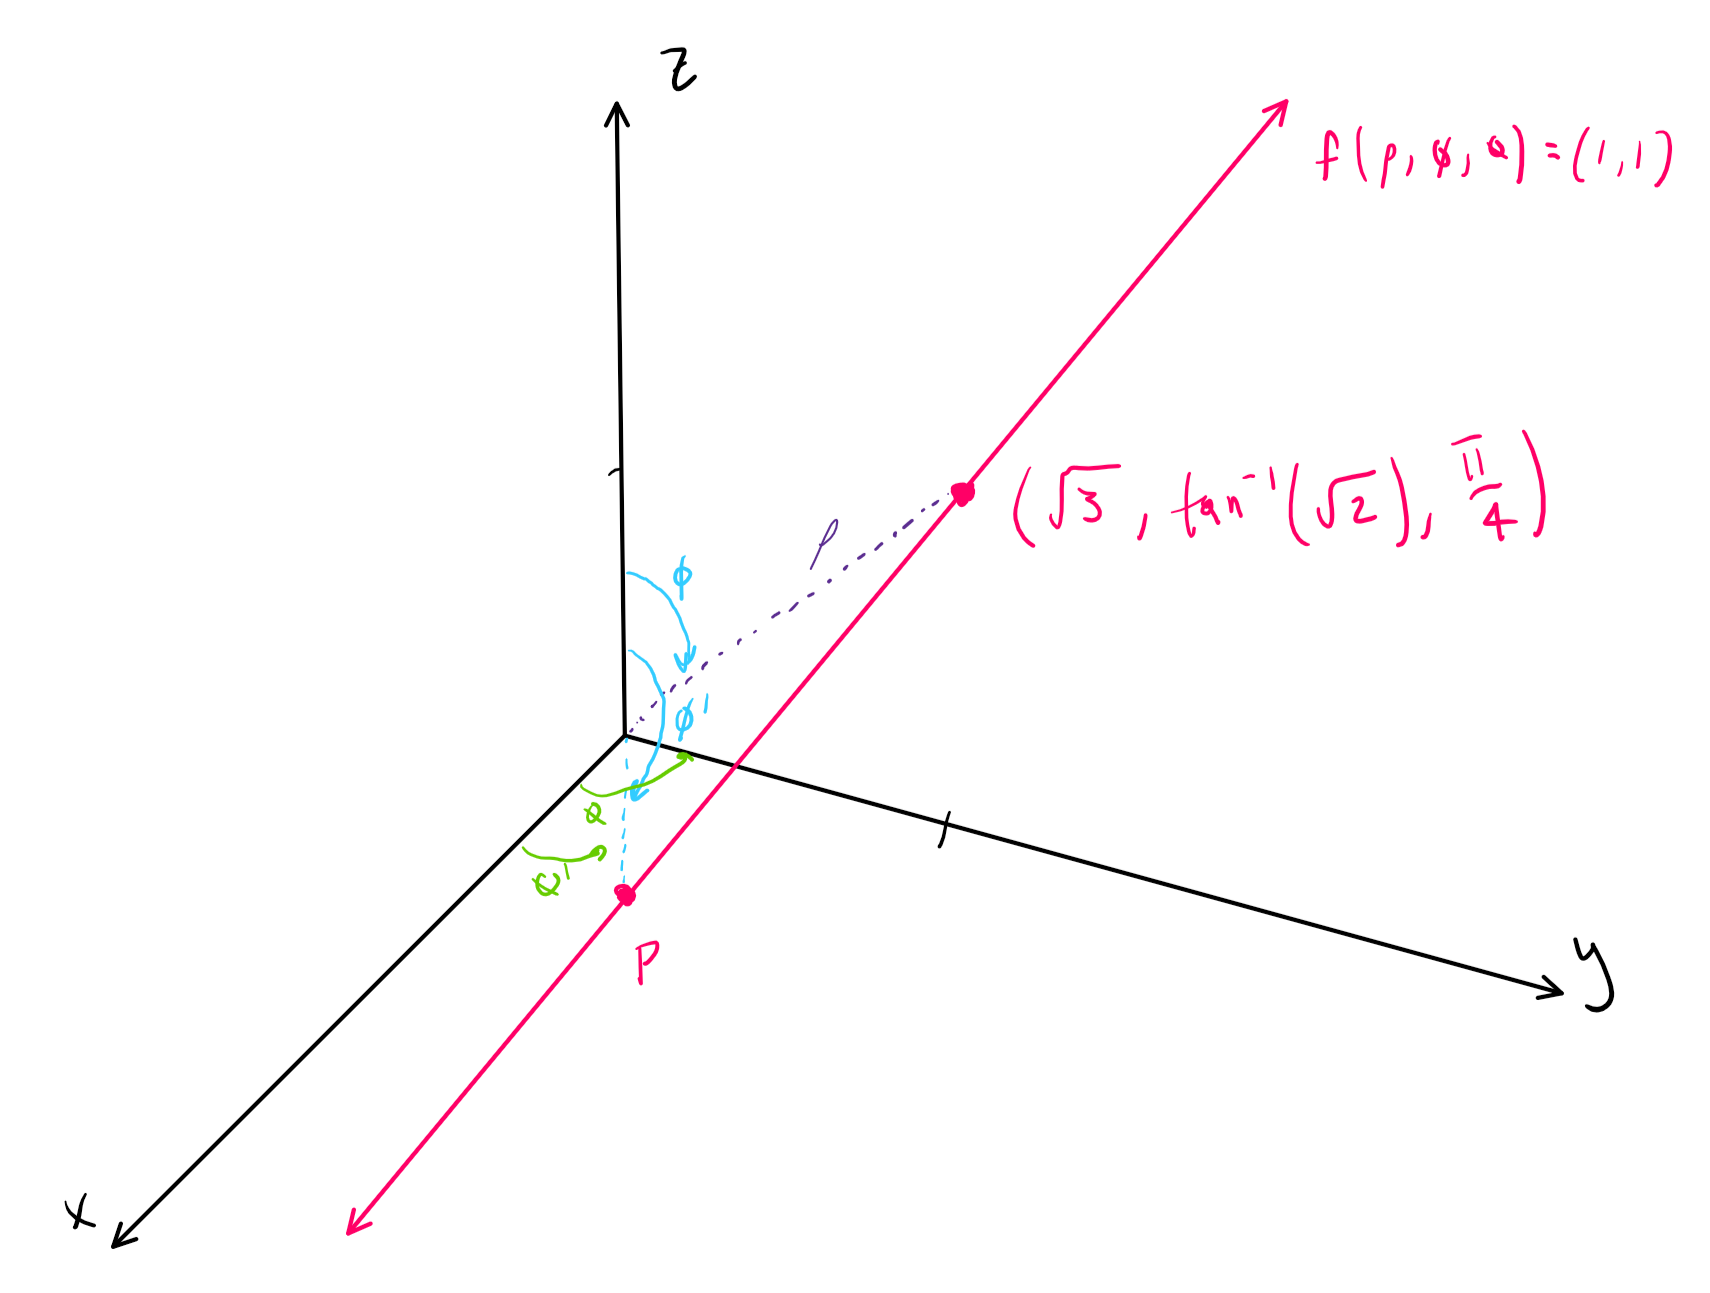
\includegraphics[scale=.5]{hw 6 (1).PNG}
    \end{center}
    
    Note, the point $P$ is after our change in $x$. So, $\phi'(\sqrt{3}) = \frac{\sqrt{6}}{6} > 0$ and $\theta'(\sqrt{3}) = -\frac{\sqrt{3}}{2} < 0$, which makes sense because when $\rho$ increases, then $\theta$ decreases and $\phi$ increases, which is what the math tells us.
\end{itemize}
\end{problem}


\begin{problem}{24}
Consider the equation $xe^y + ye^x = 0$. 

\begin{itemize}
    \item[(a)] Prove that this equation defines $y$ as a $C^\infty$ function of $x$ in a neighborhood of $(0,0)$.
    
    \begin{sol}
    Let $f : \mathbb{R}^2 \to \mathbb{R}$ be defined by $f(x,y) = xe^y + ye^x$. Then, $D_1f(x,y) = e^y + ye^x$, $D_{1,1}f(x,y) = ye^x$, $D_2f(x,y) = xe^y + e^x$, $D_{2,2}f(x,y) = xe^y$, and $D_{1,2}f(x,y) = e^y+e^x$.
    
    \vspace{1em}
    
    Let $P(n)$ be the statement "$\frac{\partial^n f}{\partial y^n}(x,y) = xe^y$".
    
    \underline{Base Case}: $\frac{\partial^2 f}{\partial y^2} = xe^y$. Thus, the base case is true. 
    
    \underline{Inductive Step}: Suppose $P(k)$ is true for some $k \geq 2$. Then, $\frac{\partial^k f}{\partial y^k}(x,y) = xe^y$, which implies $\frac{\partial^{k+1}f}{\partial y^{k+1}}(x,y) = xe^y$. So, $P(k+1)$ is true.
    
    \vspace{1em}
    
    Now, let $P(n)$ be the statement "$\frac{\partial^n f}{\partial x^n}(x,y) = ye^x$".
    
    \underline{Base Case}: $\frac{\partial^2 f}{\partial x^2}(x,y) = ye^x$. Thus, the base case is true. 
    
    \underline{Inductive Step}: Suppose $P(k)$ is true for some $k \geq 2$. Then, $\frac{\partial^k f}{\partial x^k}(x,y) = ye^x$, which implies $\frac{\partial^{k+1}f}{\partial x^{k+1}}(x,y) = ye^x$. So, $P(k+1)$ is true. Let $m \geq 2$ be arbitrary but fixed. Then, $\frac{\partial^m f}{\partial y^m}(x,y) = xe^y$ implies $\frac{\partial^{m+1} f}{\partial y^mx}(x,y) = e^y$. Also, $\frac{\partial^m f}{\partial x^m}(x,y) = ye^x$ implies $\frac{\partial^{m+1} f}{\partial x^my}(x,y) = e^x$. 
    
    \vspace{1em}
    
    Lastly, let $P(n)$ now be the statement "$\frac{\partial^{m+n} f}{\partial x^my^n}(x,y) = 0$. 
    
    \underline{Base Case}: $\frac{\partial^{m+1} f}{\partial x^my} = e^x$, which implies $\frac{\partial^{m+2} f}{\partial x^my^2}(x,y) = 0$. Thus, the base case is true. 
    
    \underline{Inductive Step}: Suppose $P(k)$ is true for some $k \geq 2$. Then, $\frac{\partial^{m + k} f}{\partial x^my^k}(x,y) = 0$, which implies $\frac{\partial^{m+k+1}f}{\partial x^my^{k+1}} = 0$. So, $P(k+1)$ is true.
    
    \hspace{1em} In total, we have $\frac{\partial f}{\partial x}(x,y) = e^y + ye^x$, $\frac{\partial f}{\partial y}(x,y) = xe^y + e^x$, $\frac{\partial^n f}{\partial x^n}(x,y) = ye^x$, $\frac{\partial^{n+1} f}{\partial x^n}(x,y) = e^x$, $\frac{\partial^n f}{\partial y^n}(x,y) = xe^y$, $\frac{\partial^{n+1} f}{\partial y^n}(x,y) = e^y$, and $\frac{\partial^{m+n} f}{\partial x^my^n}(x,y) = 0$ for all $n,m \geq 2$. Clearly, they are all continuous. Therefore, $f$ is $C^\infty$. Note, $f(0,0) = 0$ and $D_2f(0,0) = 1 \neq 0$, so by the implicit function theorem, there exists $r,s > 0$ and $g : B_s(0) \to B_r(0)$ defined by $f(x,g(x)) = 0$. Therefore, $f$ and $g$ are $C^\infty$ and $f(x,y) = 0$ defines $y$ as a $C^\infty$ function of $x$ in a neighborhood of $(0,0)$.
    \end{sol}
    
    \item[(b)] Let $y = g(x)$ be this implicitly defined function. Find $g'(0)$ and $g''(0)$.
    
    \begin{sol}
    Note, $$g'(x) = -\frac{D_1f}{D_2f} = -\frac{e^y+ye^x}{xe^y+e^x}$$ and 
    \begin{align*}
        g''(x) &= \frac{-(\frac{\partial f}{\partial y})^2\frac{\partial^2 f}{\partial x^2} + 2\frac{\partial f}{\partial x}\frac{\partial f}{\partial y}\frac{\partial^2 f}{\partial xy}-(\frac{\partial f}{\partial x})^2\frac{\partial^2 f}{\partial y^2}}{(\frac{\partial f}{\partial y})^3} \\ &= \frac{-(xe^y+e^x)^2(ye^x)+2(e^y+ye^x)(xe^y+e^x)(e^y+e^x)-(e^y+ye^x)^2(xe^y)}{(xe^y+e^x)^3}.
    \end{align*}
    So, from evaluating, we get $g'(0) = -1$ and $g''(0) = -4$.
    \end{sol}
    
    \item[(c)] Use this information to explain the appearance of the curve $xe^y + ye^x = 0$ near $(0,0)$.
    As $(x,y)$ approaches $(0,0)$, the slope is directed downward at a decreasing rate.
\end{itemize}
\end{problem}

\begin{problem}{25}
  Let $p,q \geq 1$ with $\frac{1}{p} + \frac{1}{q} = 1$. \begin{itemize}
      \item[(a)] Use the method of Lagrange multipliers to find the minimum of $\frac{1}{p}x^p + \frac{1}{q}y^q$ subject to the constraints $xy = 1$ and $x > 0$.
      
      \begin{sol}
      Taking each partial derivative, we must find a Lagrange multiplier $\lambda$ such that \begin{align}
          x^{p-1} - \lambda y &= 0 \\ y^{q-1} - \lambda x &= 0.
      \end{align} Note, $x = \frac{1}{y}$ and $y = \frac{1}{x}$. So, adding $\lambda y$ and multiplying by $x$, or $\frac{1}{y}$, to equation (1), we get $x^p = \lambda$. Similarly with equation (2), we get $y^q = \lambda$. Since $xy = 1$, then $x = y = 1$. Therefore, the minimum of $\frac{1}{p}x^p + \frac{1}{q}y^q$ subject to the constraints $xy = 1$ and $x > 0$ with $p,q \geq 1$ and $\frac{1}{p} + \frac{1}{q} = 1$ is $\frac{1}{p} + \frac{1}{q} = 1$.
      \end{sol}
      
      \item[(b)] Prove that $\frac{1}{p}x^p + \frac{1}{q}y^q \geq xy$ for all $x,y \geq 0$.
      
      \begin{sol}
      Clearly, it is true if either $x$ or $y$ are zero, so suppose $x$ and $y$ are greater than zero. Note, if $(x,y)$ satisfy the inequality, then all numbers of the form $xr^{\frac{1}{p}}$ and $yr^{\frac{1}{q}}$ are true for any $r \in \mathbb{R}^+$. Thus, we may restrict ourselves such that $xy = 1$, which implies we want to show that for all $x,y \in \mathbb{R}^+$ with $xy=1$, we get $$\frac{1}{p}x^p + \frac{1}{q}y^q \geq 1.$$ 
      
      \hspace{1em} So, we must see if the minimum of $\frac{1}{p}x^p + \frac{1}{q}y^q$ subject to the constraints exists. This is exactly part (a). Thus, $\frac{1}{p}x^p + \frac{1}{q}y^q \geq xy$ for all $x,y \geq 0$.
      \end{sol}
      
      \item[(c)] Prove H\"older's inequality: if $u_i, v_i \geq 0$ for $i = 1, \dots, n$, then $$\sum_{i = 1}^nu_iv_i \leq \left( \sum_{i = 1}^n u_i^p \right)^{\frac{1}{p}} \left( \sum_{i = 1}^n v_i^q \right)^{\frac{1}{q}}.$$ (Hints: for $u = (u_1, \dots, u_n)$ let $\lVert u \rVert_p = \left( \sum_{i = 1}^n u_i^p \right)^{\frac{1}{p}}$ . If $\lVert u \rVert_p, \lVert v \rVert_q \neq 0$, let $x = \frac{u_i}{\lVert u \rVert_p}$ and $\frac{v_i}{\lVert v \rVert_q}$ in part (b).)
      
      \begin{sol}
      Let $$u = \frac{u_i}{\left( \sum_{i = 1}^n u_i^p \right)^{\frac{1}{p}}} \hspace{2em} \text{and} \hspace{2em} v = \frac{v_i}{\left( \sum_{i = 1}^n v_i^q \right)^{\frac{1}{q}}},$$ such that $u_1,u_2,\dots,u_n,v_1,v_2,\dots,v_n \in \mathbb{R}^+$ and each component of $(u,v)$ nonzero. Then, by Young's inequality, which is part (b), we get
      \begin{align*}
          \sum_{i = 1}^n \left| u_iv_i \right| &\leq \sum_{i = 1}^n \left( \frac{u_i^p}{p} + \frac{v_i^q}{q} \right).
      \end{align*}
      Using the fact that $\frac{1}{p} + \frac{1}{q} = 1$, we get $\sum_{i = 1}^n \left| u_iv_i \right| \leq 1$. One can also show that $\sum_{i = 1}^nu_i^p = 1$ and $\sum_{i = 1}^nv_i^p = 1$. Therefore, we get H\"older's inequality $$\sum_{i = 1}^nu_iv_i \leq \left( \sum_{i = 1}^n u_i^p \right)^{\frac{1}{p}} \left( \sum_{i = 1}^n v_i^q \right)^{\frac{1}{q}}.$$
      \end{sol}
  \end{itemize}
  \end{problem}
  
  
  \begin{problem}{26}
  Let $f : \mathbb{R}^2 \to \mathbb{R}^2$ be given by $f(x) = (e^{x_1}\cos x_2,e^{x_1}\sin x_2).$ \begin{itemize}
      \item[(a)] Find (with proof) the range of $f$.
      
      \begin{sol}
      Consider the following sets: $Z_1 = \mathbb{R}_* \times \mathbb{R}$ and $Z_2 = \mathbb{R} \times \mathbb{R}_*$. For $a \in Z_1$ or $a \in Z_2$, let $g_1 : Z_1 \to \mathbb{R}_*^2$ be defined by $g_1(a) = f(b_1,b_2)$ and let $g_2 : Z_2 \to \mathbb{R}_*^2$ be defined by $g_2(a) = f(b_1,b_2)$, respectively such that $b_1 = \ln \left( \sqrt{a_1^2 + a_2^2} \right)$ and $$b_2 = \begin{cases} 
        \tan^{-1} \left( \frac{a_2}{a_1} \right), & \text{if } a_1 \neq 0 \\
        \cot^{-1}\left( \frac{a_1}{a_2} \right), & \text{if } a_2 \neq 0.
     \end{cases}$$
     \hspace{1em} Without loss of generality, since it can be shown similarly in both cases, let $a \in Z_1$. Then, \begin{align*}
         g_1(a) &= f(b_1,b_2) \\ 
         &= \left( e^{\ln \left( \sqrt{a_1^2 + a_2^2} \right)}\cos \left( \tan^{-1} \left( \frac{a_2}{a_1} \right) \right), e^{\ln \left( \sqrt{a_1^2 + a_2^2} \right)}\sin \left( \tan^{-1} \left( \frac{a_2}{a_1} \right) \right) \right)\\ 
         &= \left( \sqrt{a_1^2 + a_2^2} \left( \frac{a_1}{\sqrt{a_1^2 + a_2^2}} \right) , \sqrt{a_1^2 + a_2^2} \left( \frac{a_2}{\sqrt{a_1^2 + a_2^2}} \right) \right) \\ 
         &= (a_1,a_2).
     \end{align*}
     Thus, $f$ is surjective if we consider the codomain to be $\mathbb{R}_*^2$. 
     Also, clearly, we cannot have $0 \in \text{ran}f$ since $e^{x_1} > 0$ for all $x_1 \in \mathbb{R}$ and if $\sin x_2 = 0$, then $\cos x_2 \neq 0$. Therefore, exhausting all possibilities, we have $\text{ran}f = \mathbb{R}_*^2$.
      \end{sol}
      
      \item[(b)] Prove that $f'(x)$ is non-singular for every $x \in \mathbb{R}^2$, but that $f$ is not one-to-one.
      
      \begin{sol}
      Let $f : \mathbb{R}^2 \to \mathbb{R}^2$ be defined by $f(x) = (e^{x_1}\cos x_2,e^{x_1} \sin x_2)$. Then, $$f'(x) = \begin{pmatrix}
          e^{x_1} \cos x_2 & -e^{x_1} \sin x_2 \\ 
          e^{x_1} \sin x_2 & e^{x_1} \cos x_2
      \end{pmatrix}.$$ Now, \begin{align*}
          \left| \begin{pmatrix}
          e^{x_1} \cos x_2 & -e^{x_1} \sin x_2 \\ 
          e^{x_1} \sin x_2 & e^{x_1} \cos x_2
      \end{pmatrix} \right| &= e^{2x_1} \cos^2 x_2 + e^{2x_1} \sin^2 x_2 \\ &= e^{2x_1}.
      \end{align*}
      Since $e^{2x_1} > 0$ for all $x_1 \in \mathbb{R}$, then $f'(x)$ is always non-singular. Also, since neither $\cos$ nor $\sin$ are injective on $\mathbb{R}$, then $f$ is not injective.
      \end{sol}
      
      \item[(c)] Let $U = \{x \in \mathbb{R}^2 : \left| x_2 \right| < \pi \}$. Prove that $\restr{f}{U}$ is one-to-one, and find $f(U)$. Also prove that for any open set $V$ properly containing $U$, $\restr{f}{V}$ is not one-to-one.
      
      \begin{sol}
      Let $U = \{x \in \mathbb{R}^2 : \left| x_2 \right| < \pi \} = \{x \in \mathbb{R}^2 : x_2 \in (-\pi,\pi)\}$. Let $x,y \in U$ such that $f(x) = f(y)$. Then, 
      \begin{align*}
         e^{x_1}\cos x_2 &= e^{y_1}\cos y_2 &\hspace{3em} e^{x_1}\sin x_2 &= e^{y_1}\sin y_2 \\ e^{2x_1}\cos^2 x_2 &= e^{2y_1}\cos^2 y_2 &\hspace{3em} e^{2x_1}\sin^2 x_2 &= e^{2y_1}\sin^2 y_2. \tag*{(By squaring both sides)}
      \end{align*} 
      By adding the two equations together, we get $$e^{2x_1}\cos^2 x_2 + e^{2x_1}\sin^2 x_2 = e^{2y_1}\cos^2 y_2 + e^{2y_1}\sin^2 y_2,$$ which simplifies to $e^{2x_1} = e^{2y_1}$. These are injective functions, which implies $x_1 = y_1$. By substitution, we get $e^{x_1}\cos x_2 = e^{x_1}\cos y_2$ and $e^{x_1}\sin x_2 = e^{x_1}\sin y_2$. By division, we have $\cos x_2 = \cos y_2$ and $\sin x_2 = \sin y_2$. This is broken down in the following cases:
      
      \begin{itemize}
          \item[\underline{Case 1:}] $x_2 \in (-\pi,0)$:
          \begin{itemize}
              \item[\underline{Case 1a:}] Let $y_2 \in (-\pi,0)$. Note, $\cos$ is injective on this interval, so $\cos x_2 = \cos y_2$ implies $x_2 = y_2$.
              
              \item[\underline{Case 1b:}] Let $y_2 \in [0,\pi)$. Since $\sin x_2 < 0$ and $\sin y_2 \geq 0$, then $\sin x_2 \neq \sin y_2$, which is impossible.
          \end{itemize}
          
          \item[\underline{Case 2:}] $x_2 \in [0,\pi)$:
          \begin{itemize}
              \item[\underline{Case 1a:}] Let $y_2 \in (-\pi,0)$. Since $\sin x_2 \geq 0$ and $\sin y_2 < 0$, then $\sin x_2 \neq \sin y_2$, which is impossible.
              
              \item[\underline{Case 1b:}] Let $y_2 \in [0,\pi)$. Note, $\cos$ is injective on this interval, which implies $\cos x_2 = \cos y_2$, which implies $x_2 = y_2$.
          \end{itemize}
      \end{itemize}
      
      So, in all possible cases, we have $x_2 = y_2$. Therefore, $x = y$. Thus, $\restr{f}{U}$ is injective.
      
      \hspace{1em}Now, let $a \in \mathbb{R}_*^2$. Also, let $b_1 = \ln \left( \sqrt{a_1^2 + a_2^2} \right)$ and $$b_2 = \begin{cases} 
        \tan^{-1} \left( \frac{a_2}{a_1} \right), & \text{if } a_1 \neq 0 \\
        \cot^{-1}\left( \frac{a_1}{a_2} \right), & \text{if } a_2 \neq 0.
     \end{cases}$$ Note, $b \in U$ since the range of $\tan^{-1}$ and $\cot^{-1}$ is $(\frac{-\pi}{2},\frac{\pi}{2})$. From (a), we know that $f(b) = a$. So, $\text{ran}\left(\restr{f}{U}\right) \supseteq \mathbb{R}_*^2$.However, the cardinality of the range cannot be larger when the domain is restricted. Thus, $$\text{ran}\left(\restr{f}{U}\right) = \mathbb{R}_*^2.$$
     
     \hspace{1em} Now, suppose $V \subseteq \mathbb{R}^2$ open such that $U \subset V$. Then, there exists $q \in V \setminus U$. Let $$E = \begin{cases} 
        \{q_2 + 2\pi k : k \in \mathbb{Z},q_2 \geq q_2 + 2\pi k > -\pi\}, & \text{if } q_2 \geq \pi \\
        \{q_2 + 2\pi k : k \in \mathbb{Z},\pi > q_2 + 2 \pi k \geq q_2\}, & \text{if } q_2 \leq -\pi.
     \end{cases}$$
      \hspace{1em} Suppose, without loss of generality, that $q_2 \geq \pi$. Now, $E$ is finite and $E \neq \emptyset$, since $q_2 \in E$. Let $m = \min E$. Then, if $m \not \in U$, then $m = \pi$, else $m - 2\pi \in E$, which is a contradiction. If $m \in U$, let $u_2 = m$ with $u \in U$. Else, there exists $r > 0$ such that $B_r(q_1,q_2) \subseteq V$ since $V$ is open.
      
      \hspace{1em} Let $p = \min\{q_2 + \frac{r}{2}, q_2 + \frac{3\pi}{2}\}$. So, $(q_1,p) \in V$. Also, there exists $k \in \mathbb{Z}$ such that $q_2 + 2 \pi k = m$ since $m \in E$, which implies $$\pi = m = q_2 + 2 \pi k < p + 2 \pi k \leq q_2 + \frac{3\pi}{2} + 2\pi k = m + \frac{3 \pi}{2} = \frac{5 \pi}{2}.$$ By subtracting $2 \pi$, we get $-\pi < p + 2 \pi (k-1) \leq \frac{3 \pi}{2}$, which implies $(q_1,p+2\pi (k-1)) \in U$. If this is the case, let $u_2 = p + 2 \pi (k-1)$. Either way, we have $(q_1,u_2) \in V$ and $(q_1,u_2 + 2 \pi \alpha) \in U \subset V$ for some $\alpha \in \mathbb{Z}$. So, \begin{align*}
          f(q_1,u_2) &= (e^{q_1}\cos u_2, e^{q_1} \sin u_2) \\ &= (e^{q_1} \cos (u_2 + 2 \pi \alpha),e^{q_1} \sin (u_2 + 2 \pi \alpha)) \\ &= f(q_1,u_2 + 2\pi \alpha).
      \end{align*}
      Therefore, $\restr{f}{V}$ is not injective.
      \end{sol}
  \end{itemize}
  \end{problem}
  
  
  \begin{problem}{27}
  Let $f : \mathbb{R}^2 \to \mathbb{R}$ be continuously differentiable. In each part, the portion of the level set $\{x \in \mathbb{R}^2 : f(x) = 0\}$ is sketched near a point on the level set. What can you say about the derivatives $f'(A)$ and $f'(B)$? Justify your answers precisely.
  
  \begin{center}
      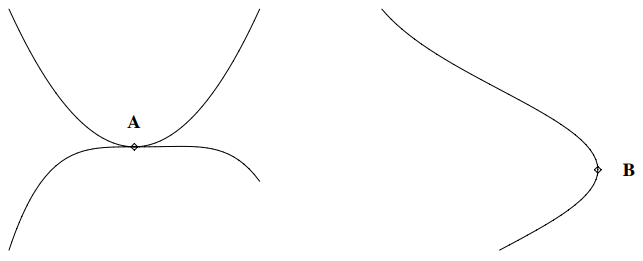
\includegraphics[scale=1]{473figure.PNG}
      \end{center}
      
      \begin{sol}
      Note, the important thing to consider with the two diagrams is whether, for $x = (x_1,x_2) \in \mathbb{R}^2$, $x_1$ can be represented as a function of $x_2$ or if $x_2$ can be represented as a function of $x_1$. Considering the diagram with point $A$, there clearly does not exist a function that can approximate one variable with the other. Thus, $D_1f(A) = D_2f(A) = 0$. As for the diagram with point $B$, $x_1$ can be represented as a function of $x_2$, but $x_2$ can not be represented as a function of $x_1$. Therefore, $D_2f(B) = 0$.
      \end{sol}
  \end{problem}
  
  
  \begin{problem}{28}
  Let $f : U \subseteq \mathbb{R}^3 \to \mathbb{R}^2$ be continuously differentiable, let $a \in U$, and suppose that $\frac{\partial f}{\partial (x_2,x_3)}(a)$ is non-singular (as a $2 \times 2$ matrix). Prove that there are open subsets $V$ and $W$ of $\mathbb{R}^3$ with $a \in W$, and a $C^1$-diffeomorphism $h : V \to W$, such that $f \circ h(x) = (x_2, x_3)$ for all $x \in V$. (Hint: let $F(x) = (x_1,f(x))$ and use the inverse function theorem.)
  \end{problem}
  
  \begin{sol}
  Let $f : U \subseteq \mathbb{R}^3 \to \mathbb{R}^2$ be continuously differentiable, let $a \in U$, and suppose that $\frac{\partial f}{\partial (x_2,x_3)}(a) \in M_2$ is non-singular. Define $F : \mathbb{R}^3 \to \mathbb{R}^3$ by $F(x) = (x_1,f(x))$. Since $\frac{\delta f}{\delta (a_2,a_3)}$ is invertible, then by the implicit function theorem, there exists $r,s > 0$ such that $B_r(a_2,a_3) \subseteq U$, $\frac{\delta f}{\delta (x_2,x_3)}$ is invertible for all $(x_2,x_3) \in B_r(a_2,a_3)$, and for each $x_1 \in B_s(a_1)$, there exists a unique $h(x) \in B_r(a)$.
  \end{sol}

\begin{problem}{29}
  Let $f : [a,b] \to \mathbb{R}$ and let $c \in [a,b].$ Recall that the \textit{oscillation of f at c} is the quantity $$\text{osc}(f,c) = \lim_{r \to 0^+} \left( \sup_{x,y \in B_r(c) \cap [a,b]} \left| f(x) - f(y) \right| \right).$$ 
  Prove that $f$ is continuous at $c$ if and only if $\text{osc}(f,c) = 0$.
  \end{problem}
  \begin{sol}
  Let $f : [a,b] \to \mathbb{R}$ and $c \in (a,b)$. 
  
  $(\Longrightarrow):$ Let $f$ be continuous at $c$. Let $\epsilon > 0$ be arbitrary but fixed. Then, there exists $r > 0$ such that for $x,y \in B_r(c)$, we have $\left| f(x) - f(c) \right| < \frac{\epsilon}{2}$ and $\left| f(y) - f(c) \right| < \frac{\epsilon}{2}$, which from the triangle inequality implies $$\left| f(x) - f(y) \right| \leq \left| f(x) - f(c) \right| + \left| f(y) - f(c) \right| < \epsilon.$$ Thus, $$\lim_{r \to 0^+} \left( \sup_{x,y \in B_h(c) \cap [a,b]} \left| f(x) - f(y) \right| \right) \leq \epsilon \hspace{1em} \text{if} \hspace{1em} h < r.$$ This implies $\text{osc}(f,c) = 0$.
  
  $(\Longleftarrow):$ Let $\text{osc}(f,c) = 0$ and $\epsilon > 0$ be arbitrary but fixed. Then, $$\lim_{r \to 0^+} \left( \sup_{x,y \in B_r(c) \cap [a,b]} \left| f(x) - f(y) \right| \right) < \epsilon$$ for some $r > 0$.
  So, $\left| f(x) - f(y) \right| < \epsilon$ if $x,y \in B_r(c)$. If $c = y$, then $\left| f(x) - f(c) \right| < \epsilon$. Therefore, $f$ is continuous at $c$.
  
  This argument is similar if $c = a$ or $c = d$.
  \end{sol}
  
  
  \begin{problem}{30}
  Let $f$ be as in the previous problem, and let $L > 0$. Prove that the set $\{z \in [a,b] : \text{osc}(f,z) \geq L \}$ is a closed set.
  \end{problem}
  \begin{sol}
  Let $f : [a,b] \to \mathbb{R}$ and $L > 0$. Define $A = \{z \in [a,b] : \text{osc}(f,z) \geq L\}$. Notice that $A^c = (-\infty,a) \cup \{z \in [a,b] : \text{osc}(f,z) < L\} \cup (b,\infty)$. Then we have the following cases.
  
  \begin{itemize}[leftmargin=.6in]
      \item[\underline{Case 1:}] Let $c \in (-\infty,a) \cup (b,\infty)$. Then, since $(-\infty,a) \cup (b,\infty)$ is open, then there exists $r_0 > 0$ such that $B_{r_0}(c) \subseteq A^c$.
      
      \item[\underline{Case 2:}] Let $c \in \{z \in [a,b] : \text{osc}(f,z) < L\}$. Then, there must exist $\delta > 0$ such that for all $r \in (0,\delta)$, then $$\sup_{x,y \in B_r(c) \cap [a,b]} \left| f(x) - f(y) \right| < L.$$ 
      Let $d \in [a,b]$. Fix $r \in (0,\delta)$. Let $d \in B_{\frac{r}{2}}(c)$. Clearly, if $d \not\in [a,b]$, then we have $d \in (-\infty, a) \cup (b,\infty) \subseteq A^c$. Suppose $d \in [a,b]$. Let $x \in B_{\frac{r}{2}}(d) \cap [a,b]$. This gives us \begin{align*}
          \left| x - c \right| &\leq \left| x - d \right| + \left| c - d \right| \tag*{(By triangle inequality)} \\
          &< \frac{r}{2} + \frac{r}{2} \\ 
          &= r.
      \end{align*}
      So, $x \in B_r(c)$, which implies $B_{\frac{r}{2}}(d) \subseteq B_r(c)$. Thus, \begin{align} \sup_{x,y \in B_{\frac{r}{2}}(d) \cap [a,d]} \left| f(x) - f(y) \right| \leq \sup_{x,y \in B_r(c) \cap [a,b]} \left| f(x) - f(y) \right|. \end{align} We now have, \begin{align*}
          \text{osc}(f,d)
          &= \lim_{r \to \infty} \left( \sup_{x,y \in B_{\frac{r}{2}}(d) \cap [a,d]} \left| f(x) - f(y) \right| \right) \tag*{(Definition of oscillation of $f$ at $d$)} \\
          &\leq \lim_{r \to \infty} \left( \sup_{x,y \in B_r(c) \cap [a,b]} \left| f(x) - f(y) \right| \right) \tag*{(By (1))} \\ 
          &= \text{osc}(f,c) \tag*{(Definition of oscillation of $f$ at $c$)} \\
          &< L.
      \end{align*}
      Thus, $d \in A^c$, which implies $B_{\frac{r}{2}}(c) \subseteq A^c$. 
  \end{itemize}
   Therefore, in both cases, we have that $A^c$ is open, which implies that $A$ is closed.
  \end{sol}
  
  
  \begin{problem}{31}
  Let $[c,d]$ be a closed bounded interval, and let $(a_1,b_1),\dots,(a_n,b_n)$ be open intervals such that $[c,d] \subseteq \cup_{i = 1}^n(a_i,b_i)$. Prove that $d-c < \sum_{i = 1}^n(b_i - a_i)$. (Hints: choose $i_1$ so that $c \in (a_{i_1},b_{i_1})$. If $b_{i_1} \leq d$ choose $i_2$ so that $b_{i_1} \in (a_{i_2},b_{i_2})$. Explain why in the continuation of this process there must be $k \leq n$ such that $d \in (a_{i_k},b_{i_k})$.)
  \end{problem}
  \begin{sol}
  Let $C = [c,d]$ be a closed bounded interval and $A_1 = (a_1,b_1), \dots, A_n = (a_n, b_n)$ be open intervals such that $[c,d] \subseteq \cup_{i = 1}^nA_i$. Let $\epsilon > 0$ be arbitrary but fixed. Choose $j$ such that $Q_j = (q_j,p_j) \supseteq A_j$ with $p_j - q_j \leq (1 + \epsilon) \left| b_j - a_j \right|$. Since $\cup_{j = 1}^\infty Q_j$ is an open cover of the compact set $[c,d]$, there exists a finite subcover $[c,d] \subseteq \cup_{i = 1}^N Q_j$. By taking the closure of each $Q_j$, we have $d - c \leq \sum_{j = 1}^N (p_j - q_j)$. As a result, we have $$d - c \leq (1 + \epsilon)\sum_{j = 1}^N(b_j - a_j).$$ Since $\epsilon > 0$, then we have the strict inequality $d - c < \sum_{j = 1}^N(b_j - a_j)$.
  \end{sol}
  
  
  \begin{problem}{32}
  For this exercise you must recall the definition and properties of \textit{Lebesgue outer measure} from the notes. Let $A,B \subseteq \mathbb{R}$, and suppose that $m^*(A) = 0$. Prove that $m^*(A \cup B) = m^*(A) + m^*(B)$.
  \end{problem}
  \begin{sol}
  Let $A,B \subseteq \mathbb{R}$ and $m^*(A) = 0$. By Theorem 15.3 (2), we have $m^*(A \cup B) \leq m^*(A) + m^*(B)$. Also, \begin{align*}
      m^*(A) + m^*(B) &= 0 + m^*(B) \tag*{(By monotonicity of the outer measure)} \\ &= m^*(B) \\ &\leq m^*(A \cup B). 
  \end{align*}
  So, since $m^*(A) + m^*(B) \leq m^*(A \cup B)$ and $m^*(A \cup B) \leq m^*(A) + m^*(B)$, then we must have $m^*(A \cup B) = m^*(A) + m^*(B)$.
  \end{sol}

\begin{problem}{33}
  Recall the $\textit{Borel } \sigma\textit{-algebra}$ $\mathcal{B}_\mathbb{R}$ from the course notes. Prove that $\mathcal{B}_\mathbb{R}$ is generated as a $\sigma$-algebra by the collection of closed intervals $\{[a,\infty) : a \in \mathbb{R}\}$.
  \end{problem}
  \begin{sol}
  Let $\mathcal{O}$ denote the collection of all open intervals in $\mathbb{R}$. Since every open set in $\mathbb{R}$ is at most a countable union of open intervals, Then $\mathcal{M}(\mathcal{O}) = \mathcal{B}_\mathbb{R}$. Let $\mathcal{E}$ denote the collection of intervals of the form $[a,\infty)$ for all $a \in \mathbb{R}$. Let $(a,b) \in \mathcal{O}$ for some $a,b \in \mathbb{R}$ such that $b > a$. Let $a_n = a + \frac{1}{n}$ and $b_n = b - \frac{1}{n}$. Then, $$(a,b) = \bigcup_{n = 1}^\infty[a_n,b_n) = \bigcup_{n = 1}^\infty \{[a_n,\infty) \cap [b_n,\infty)^c\},$$ which implies that $(a,b) \in \mathcal{M}(\mathcal{E})$. This means that $\mathcal{O} \subseteq \mathcal{M}(\mathcal{E})$, which implies $\mathcal{M}(\mathcal{O}) \subseteq \mathcal{M}(\mathcal{E})$. But, since every element of $\mathcal{E}$ is closed, then $\mathcal{M}(\mathcal{E}) \subseteq \mathcal{B}_\mathbb{R}$. This gives us $$\mathcal{B}_\mathbb{R} = \mathcal{M}(\mathcal{O}) \subseteq \mathcal{M}(\mathcal{E}) \subseteq \mathcal{B}_\mathbb{R}.$$ Therefore, $\mathcal{M}(\mathcal{E}) = \mathcal{B}_\mathbb{R}$.
  \end{sol}
  
  
  
  \begin{problem}{34}
  Prove that for every subset $E \subseteq \mathbb{R}$ there is a $G_\delta$-set $A$ with $E \subseteq A$ and $m^*(E) = m^*(A)$.
  \end{problem}
  
  \begin{sol}
  Let $E \subseteq \mathbb{R}$ be arbitrary. By outer-measure, there exists a collection of open intervals $I_n \subseteq \mathbb{R}$ such that $E \subseteq \cup_{n = 1}^\infty I_n$. From the result of Problem 31, this gives us $$m^*(E) \leq \sum_{n = 1}^\infty m(I_n) < m^*(E) + \frac{1}{n}.$$ Also, by countable subadditivity, $m^*(\cup_{n = 1}^\infty I_n) \leq \sum_{n = 1}^\infty m(I_n)$. Let $A = \cap_{n = 1}^\infty \cup_{n = 1}^\infty I_n$. Then, $A$ is a $G_\delta$-set. This gives us $E \subseteq A$. Then, for each $n$, we get $$m^*(E) \leq m^*(A) \leq m^*(\cup_{n = 1}^\infty I_n) \leq \sum_{n = 1}^\infty m(I_n) < m^*(E) + \frac{1}{n}.$$ Therefore, by squeeze theorem, as $n$ approaches $\infty$, then $m^*(E) = m^*(A)$.
  \end{sol}
  
  %\begin{sol}
  %Let $E \subseteq \mathbb{R}$ be arbitrary. For each $i \in \mathbb{Z}^+$, there exists $A_i$ open such that $E \subseteq A_i$. Let $$A = \bigcap_{i = 1}^\infty A_i.$$ Note, $A$ is a $G_\delta$ set and is measurable and $E \subseteq A$. 
  %\end{sol}
  
  
  
  \begin{problem}{35}
  Let $f : \mathbb{R} \to \mathbb{R}$ be a function. Let $A = \{x \in \mathbb{R} : f \text{ is continuous at } x\}$. Prove that $A$ is a $G_\delta$-set. (Hint: use the oscillation of $f$ from homework 8.)
  \end{problem}
  \begin{sol}
  Let $A = \{x \in \mathbb{R} : f \text{ is continuous at } x\}$. Note, $f$ is continuous at $c$ if and only if $\text{osc}(f,c) = 0$. That is, $f$ is continuous at $c$ if and only if \begin{align*}
      \limsup\limits_{x\to c}f(x) = \liminf\limits_{x \to c}f(x). 
  \end{align*}
  So, by looking at the complement of $A$, we get \begin{align*}
      A^c &= \left\{x \in \mathbb{R} : \liminf\limits_{x \to c}f(x) < \limsup\limits_{x\to c}f(x)\right\} \\
      &= \left\{ x \in \mathbb{R} : \exists a,b \in \mathbb{Q} \text{ s.t. } \liminf\limits_{x \to c}f(x) \leq a < b \leq \limsup\limits_{x\to c}f(x) \right\} \\
      &= \bigcup_{a,b} \left( \left\{ x \in \mathbb{R} : \liminf\limits_{x \to c}f(x) \leq a \right\} \bigcap \left\{ x \in \mathbb{R} : b \leq \limsup\limits_{x\to c}f(x) \right\} \right). \tag*{(with $a < b$)}
  \end{align*}
  \hspace{1em}Note, if $\liminf\limits_{x \to c}f(x) > a$, then there must exist $\epsilon > 0$ arbitrary but fixed such that $\inf_{\left| x - c \right| < \epsilon}f(x) > a$. Now, for each $x \in B_\epsilon(c)$, there is $\epsilon_0 > 0$ arbitrary but fixed such that $B_{\epsilon_0}(x) \subset B_\epsilon(c)$. So, we get $$\inf_{\left| x - c' \right| < \epsilon_0}f(x) \geq \inf_{\left| x - c \right| < \epsilon}f(x) > a.$$ This means that $\left\{ x \in \mathbb{R} : \liminf\limits_{x \to c}f(x) > a \right\}$ is open, which implies $\left\{ x \in \mathbb{R} : \liminf\limits_{x \to c}f(x) \leq a \right\}$ is closed. We can similarly show that $\left\{ x \in \mathbb{R} : b \leq \limsup\limits_{x\to c}f(x) \right\}$ is closed since $\limsup\limits_{x\to c}f(x) = - \left( \liminf\limits_{x \to c}(-f(x)) \right)$.
  
  Finally, since each set in the pair of a countable union defined above is closed, then $A^c$ is a $F_\sigma$-set, which implies $A$ is a $G_\delta$-set.
  \end{sol}
  
  
  
  \begin{problem}{36}
  For subsets $A,B \subseteq \mathbb{R}$ recall that the \textit{distance} between $A$ and $B$ is defined to be $\text{dist}(A,B) = \text{inf}\{ \left| x - y \right| : x \in A, y \in B \}$. Let $A$ and $B$ be subsets of $\mathbb{R}$ such that $\text{dist}(A,B) > 0$. Prove that $m^*(A \cup B) = m^*(A) + m^*(B)$. 
  %(Hint: first prove the following lemma:
  \end{problem}
  \begin{sol}
  Let $A,B \subseteq \mathbb{R}$. Let $\epsilon > 0$ be arbitrary but fixed such that $\text{dist}(A,B) \geq \epsilon$. Let $E = \cup_{x \in A}B_{\frac{\epsilon}{2}}(x)$. Then, $A \subset E$. Also, since $E$ used the ball of radius $\frac{\epsilon}{2}$, then $E \cap B = \emptyset$. Also, since $E$ used a countable union of open balls, then $E$ is measurable. This gives us $m^*(A \cup B) = m^*((A \cup B) \cap E) + m^*((A \cup B) \cap E^c)$ from Definition 17.1 in the notes. But, note that $(A \cup B) \cap E^c = B$ and $(A \cup B) \cap E = A$. Therefore, we have $m^*(A \cup B) = m^*(A) + m^*(B)$.
  \end{sol}
  
  %\begin{lemma}{1}
  %Let $-\infty < a < b < \infty$ and let $\epsilon > 0$. There are open intervals $I_1, \dots, I_n$ such that 
  %\begin{itemize}
  %    \item $(a,b) = \cup_{i = 1}^nI_i$
      
  %    \item $\sum_{i = 1}^n \left| I_i \right| < b - a + \epsilon$ (where $\left| I \right|$ denotes the length of the interval $I$)
      
  %    \item $\left| I_i \right| < \epsilon$ for $1 \leq i \leq n$
  %\end{itemize}
  %\end{lemma}

  \begin{problem}{37}
    Let $A_1,A_2,\dots$ be measurable sets, and suppose that $A_1 \subseteq A_2 \subseteq A_3 \subseteq \dots$. Prove that $m(\cup _{n = 1}^{\infty}A_n) = \lim_{n \to \infty}m(A_n)$. (This is called \textit{continuity from below} of Lebesgue measure.) (Hints: use Proposition 16.4 of the notes. It is useful also to remember that $\sum_{n = 1}^{\infty}a_n = \lim_{n \to \infty}\sum_{i = 1}^{n}a_i$.)
  \end{problem}
  \begin{sol}
    Let $A_1,A_2,\dots$ be measurable sets, and suppose that $A_1 \subseteq A_2 \subseteq A_3 \subseteq \dots$. Suppose $\lim_{N \to \infty} \bigcup_{n = 1}^NA_n = A$. From Proposition 16.4, we know $$A = A_1 \cup \bigcup_{n = 1}^{\infty}(A_{n+1}  \setminus A_n).$$ Note, $A_1$ and $\bigcup_{n = 1}^{\infty}(A_{n+1}  \setminus A_n)$ are disjoint and $A$ is a $\sigma$-algebra. Since they are disjoint and measurable, then we have 
    \begin{align*}
      m(A) &= \sum_{n = 1}^{\infty}m(A_n \setminus A_{n-1}) \\
      &= \lim_{n \to \infty} \sum_{i = 1}^n m(A_i \setminus A_{i - 1}) \\
      &= \lim_{n \to \infty} m(A_n).
    \end{align*}
  \end{sol}
  
  \begin{problem}{38}
    Let $A_1,A_2,\dots$ be measurable sets, and suppose that $A_1 \supseteq A_2 \supseteq A_3 \supseteq \dots$. Suppose further that $m(A_1) < \infty$. Prove that $m(\cap_{n = 1}^{\infty}A_n) = \lim_{n \to \infty}m(A_n)$. Be sure to indicate where the finiteness hypothesis is used. (This is called \textit{continuity from above} of Lebesgue measure.) (Hints: as in the previous problem. Also, you will need to consider $B_{\infty} \coloneqq \cap_{n = 1}^{\infty}A_n$.) Give an example of a decreasing sequence of measurable sets of infinite measure for which the above conclusion is false. 
  \end{problem}
  \begin{sol}
    Let $A_1,A_2,\dots$ be measurable sets, and suppose that $A_1 \supseteq A_2 \supseteq A_3 \supseteq \dots$. Suppose further that $m(A_1) < \infty$ and $B_{\infty} \coloneqq \lim_{N \to \infty}\bigcap_{n = 1}^NA_n$. Note, $m(A_1 \setminus B_{\infty}) = \lim_{n \to \infty}m(A_1 \setminus A_n)$. Also, $m(B_{\infty}) \leq m(A_n) \leq m(A_1) < \infty$. So, by Problem 37, 
    \begin{align*}
      m(A_1) - m(B_{\infty}) &= m(A_1 \setminus B_{\infty}) \\
      &= \lim_{n \to \infty} m(A_1 \setminus A_n) \\
      &= m(A_1) - \lim_{n \to \infty} m(A_n).
    \end{align*}
    So, by subtracting the $m(A_1)$ terms from both sides, we get $$m(B_{\infty}) = \lim_{n \to \infty}m(A_n).$$
  \end{sol}
  
  Now, it is important that $A_k < \infty$ for some $k \in \mathbb{Z}$. For example, if not, suppose $A_n = (n,\infty)$. Then, $A_n \supseteq A_{n+1} \supseteq A_{n + 2} \supseteq \dots$ and $m(A_n) = \infty$ for each $n$, but $\bigcap_{n = 1}^{\infty}A_n = \emptyset$. So, we get $$\infty = \lim_{n \to \infty} m(A_n) \neq m(\bigcap_{n = 1}^{\infty}A_n) = 0.$$
  
  \begin{problem}{39}
    Let $E$ be a measurable set, and let $\epsilon > 0$. Prove that there are an open $U \supseteq E$ and a closed set $F \subseteq E$ such that $m(U \setminus F) < \epsilon$. Here is an outline.
  
    \begin{itemize}
      \item[(a)] Suppose that $E \subseteq [a,b]$. Use the definition of outer measure to find an open set $U \supseteq E$ with $m(U \setminus E) < \epsilon$.
      \item[(b)] Suppose that $E \subseteq [a,b]$. Apply the previous part to $[a,b] \setminus E$ to prove that there is a closed set $F \subseteq E$ with $m(E \setminus F) < \epsilon$.
      \item[(c)] For the general case let $E_n = E \cap [n,n+1]$ for $n \in \mathbb{Z}$, and apply the previous two parts with $\epsilon4^{-(|n|+1)}$. Use the fact that if $S_n \subseteq T_n$ then $(\cup_nT_n) \setminus (\cup_nS_n) \subseteq \cup_n(T_n \setminus S_n)$.
    \end{itemize}
  \end{problem}
  \begin{sol}
    Let $E$ be a measurable set with $m(E) < \infty$, and let $\epsilon > 0$ be arbitrary but fixed. Then, there are intervals $(a_n,b_n)$ with $E \subseteq \bigcup_{n = 1}^{\infty}(a_n,b_n)$ and $m(E) \leq \sum_{n = 1}^{\infty}m((a_n,b_n)) + \epsilon$. Define $U = \bigcup_{n = 1}^{\infty}(a_n,b_n)$. Then, $U \supseteq E$ is open and $m(U) \leq m(E) + \epsilon$. Now, since $m(U) < \infty$ and $m(E) < \infty$, then $m(U \setminus E) = m(U) - m(E) < \epsilon$.
    
    Then, since $E$ is measurable, then $E^c$ is measurable. So, there exists $O \supseteq E^c$ open such that $m(O \setminus E^c) \leq \epsilon$. Let $F = O^c$, which implies $F$ is closed and $F \subseteq E$. Then, $E \setminus F = O \setminus E^c$, which implies $m(E \setminus F) \leq \epsilon$. 
  
    Now, let $U \supseteq E$ open and $F \subseteq E$ be closed such that $m(U \setminus E) < \frac{\epsilon}{2}$ and $m(E \setminus F) < \frac{\epsilon}{2}$. Note, 
    \begin{align*}
      (U \setminus E) \cup (E \setminus F) &= (U \cap E^c) \cup (E \cap F^c) \\
      &= \left[(U \cap E^c) \cup E\right] \cap \left[(U \cap E^c) \cup F^c\right] \\
      &= \left[(U \cup E) \cap (E \cup E^c)\right] \cap \left[(U \cup F^c) \cap (E^c \cup F^c)\right] \\
      &= (U \cup E) \cap \left[(F \setminus U)^c \cap F^c\right] \\
      &= U \cap (\emptyset^c \cap F^c) \\
      &= U \cap F^c \\ &= U \setminus F.
    \end{align*}
    This gives us $$m(U \setminus F) = m\left( (U \setminus E \right) + m\left( (E \setminus F) \right) < \epsilon.$$
  \end{sol}
  
  \begin{problem}{40}
    The \textit{Cantor set}, $C$, is a subset of $[0,1]$ defined as follows. Let $F_0 = [0,1], F_1 = [0,\frac{1}{3}]\cup[\frac{2}{3},1]$, and in general, $F_{n+1}$ is obtained from $F_n$ by deleting the middle open third of each subinterval of $F_n$. (Thus $F_2 = [0,\frac{1}{9}]\cup[\frac{2}{9},\frac{1}{3}]\cup[\frac{2}{3},\frac{7}{9}]\cup[\frac{8}{9},1]$.) Then $C \coloneqq \cap_{n = 1}^{\infty}F_n$. Prove the following:
    \begin{itemize}
      \item[(a)] $F_n$ is the union of $2^n$ pairwise disjoint closed intervals each of length $3^{-n}$.
       
      \begin{sol}
        Clearly, they are disjoint as you are removing the open middle third of each interval, essentialy doubling the amount of intervals each iteration. Thus, there are $2^n$ disjoint intervals for $F_n$. As for the length, $F_0$ has length $3^{-0} = 1$, and through induction, one can clearly see, without loss of generality, by taking the first of the $2^n$ intervals in $F_n$, call it $A$, that $\sup\{x - 0 : x \in A\} = 3^{-n}$.
      \end{sol}
  
      \item[(b)] $m(C) = 0$.
      
      \begin{sol}
        By continuity from above of Lebesgue measure, we know that 
        \begin{align*}
          m(C) &= m\left(\bigcap_{n = 1}^{\infty}F_n\right) \\
          &= \lim_{n \to \infty} m(F_n) \\
          &= 0 \tag*{(Since $m(F_n = \left(\frac{2}{3} \right)^n)$)}.
        \end{align*}
      \end{sol}
  
      \item[(c)] $C$ is a closed set, $C$ has no isolated points, and the interior of $C$ is empty.  
      
      \begin{sol}
        Since $C$ is a countable union of closed intervals, then $C$ is closed.
      \end{sol}
    \end{itemize}
  \end{problem}

  \begin{problem}{41}
    Let $E$ be the nonmeasurable set desribed in section 18 of the notes. Prove that if $N \subseteq E$ and $N$ is measurable, then $m(N) = 0$. (Hint: imitate the second part of the proof of Theorem 18.1.)
    \end{problem}
    
    \begin{sol}
      Let $E$ be as described in section 18 of the notes. Let $N = \emptyset$. Then, $N \subseteq E$ and, trivially, $m(N) = 0$. So, there does exist a measurable subset of $E$. Now, suppose $N \subseteq E$ with $m(N) > 0$. Let $A = \mathbb{Q} \cap [0,1]$. Then, for each $x_1,x_2 \in A$, with $x_1 \neq x_2$, we know $$N + x_1 \bigcap N + x_2 = \emptyset.$$ Also, by translation invariance, $m(N) = m(N+x)$ for all $x \in A$. So, we have 
      \begin{align*}
        \sum_{n = 1}^{\infty} m(N) &= \sum_{n = 1}^{\infty} m(N + x_n) \tag*{(Each $x_n \in A$)} \\
        &= m\left( \bigsqcup_{n = 1}^{\infty} N+x_n \right) \\
        &\leq m([0,2]) \\ &= 2.
      \end{align*}
      Thus, by contradiction, since the first equivalence should clearly be infinity, we have $m(N) = 0$ for all measurable sets $N \subseteq E$.
    \end{sol}
    
    \begin{problem}{42}
    Let $A \subseteq \mathbb{R}$ be a measurable set with $m(A) > 0$. Prove that there exists a subset $B \subseteq A$ such that $B$ is not measurable. (Hint: if $E$ is the nonmeasurable set described in section 18 of the notes, then $A \subseteq \sqcup_{q \in \mathbb{Q}}(q+E)$.)
    \end{problem}
    
    \begin{sol}
      Let $A \subseteq \mathbb{R}$ with $m(A) > 0$. Without loss of generality, assume $A \subseteq [0,1]$ since if not, there is some $n \in \mathbb{Z}$ such that $m(A \cap [n,n+1]) > 0$ and by translation invariance, for $A' \coloneqq \{x-n : x \in [n,n+1]\}$, we have $A \cap A' \subseteq [0,1]$ and $m(A \cap A') > 0$. So, if $B \subseteq A \cap A'$ is nonmeasurable, then $B + n \subseteq A \cap [n,n+1] \subseteq A$ is nonmeasurable.
    
      Now, we know that $A$ is partitioned by the relation defined in section 18. By the axiom of choice, we can make a set $B \subseteq A$, which is the same as $E$ defined in section 18, which is nonmeasurable.
    \end{sol}
    
    \begin{problem}{43}
    Let $\mathcal{E}$ be a collection of Borel sets that generates $\mathcal{B}_{\mathbb{R}}$ (i.e. such that $\mathcal{M}(\mathcal{E}) = \mathcal{B}_{\mathbb{R}}$). Let $f : \mathbb{R} \to \mathbb{R}$. Prove that $f$ is measurable if and only if $f^{-1}(E)$ is measurable for all $E \in \mathcal{E}$. (Hint: show that $\{A \subseteq \mathbb{R} : f^{-1}(A)\text{ is measurable}\}$ is a $\sigma$-algebra.)
    \end{problem}
    
    \begin{sol} Suppose $\mathcal{E}$ is a collection of Borel sets that generates $\mathcal{B}_{\mathbb{R}}$.
    
      ($\Longrightarrow$): Suppose $f$ is measurable for some $E \in \mathcal{E}$. Let $$\mathcal{G} = \{A \subseteq \mathbb{R} : f^{-1}(A)\text{ is measurable}\}.$$
      Then, $\mathcal{G}$ is a $\sigma$-algebra since 
      \begin{align*}
        f^{-1}\left( \bigcup_{n \in \mathbb{N}}E_n  \right) &= \bigcup_{n \in \mathbb{N}}f^{-1}(E_n), \\
        f^{-1}\left( \bigcap_{n \in \mathbb{N}}E_n  \right) &= \bigcap_{n \in \mathbb{N}}f^{-1}(E_n), \text{ and}\\
        f^{-1}(E^c) &= \left(f^{-1}(E)\right)^c. \\
      \end{align*}
      Thus, $f^{-1}(E)$ is measurable for all $E \in \mathcal{E}$.
    
      ($\Longleftarrow$): Suppose $f^{-1}(E)$ is measurable for some $E \in \mathcal{E}$. Then, $f$ is measurable by Definition 19.1.
    \end{sol}
    
    \begin{problem}{44}
    Let $f_1,f_2,\dots : \mathbb{R} \to \mathbb{R}$ be measurable function, let $f : \mathbb{R} \to \mathbb{R}$, and suppose that $f_n \to f$ almost everywhere. Prove that $f$ is measurable.
    \end{problem}
    
    \begin{sol}
      Since $\{x \in \mathbb{R} : \lim_{n \to \infty} |f_n(x) - f(x)| \geq \epsilon \text{ } \forall \epsilon > 0\}$ is measurable with measure zero, then for $A \coloneqq \{x \in \mathbb{R} : \lim_{n \to \infty} |f_n(x) - f(x)| < \epsilon \text{ } \forall \epsilon > 0\} \subseteq \mathbb{R}$, we have 
      $$\left\{\restr{f_n}{A}(x)\right\}_{n \in \mathbb{N}} \to f$$ pointwise, which implies $f$ is measurable by Proposition 19.16.  
    \end{sol}
%%%%%%%%%%%%%%%%%%%%%%%%%%%%%%%%%%%%%%%%
%Do not alter anything below this line.
\end{document}